\chapter{Søgeprotokol} \vspace{-.75cm}
\textit{lol}
\section{TEC}\label{TEC_sog}
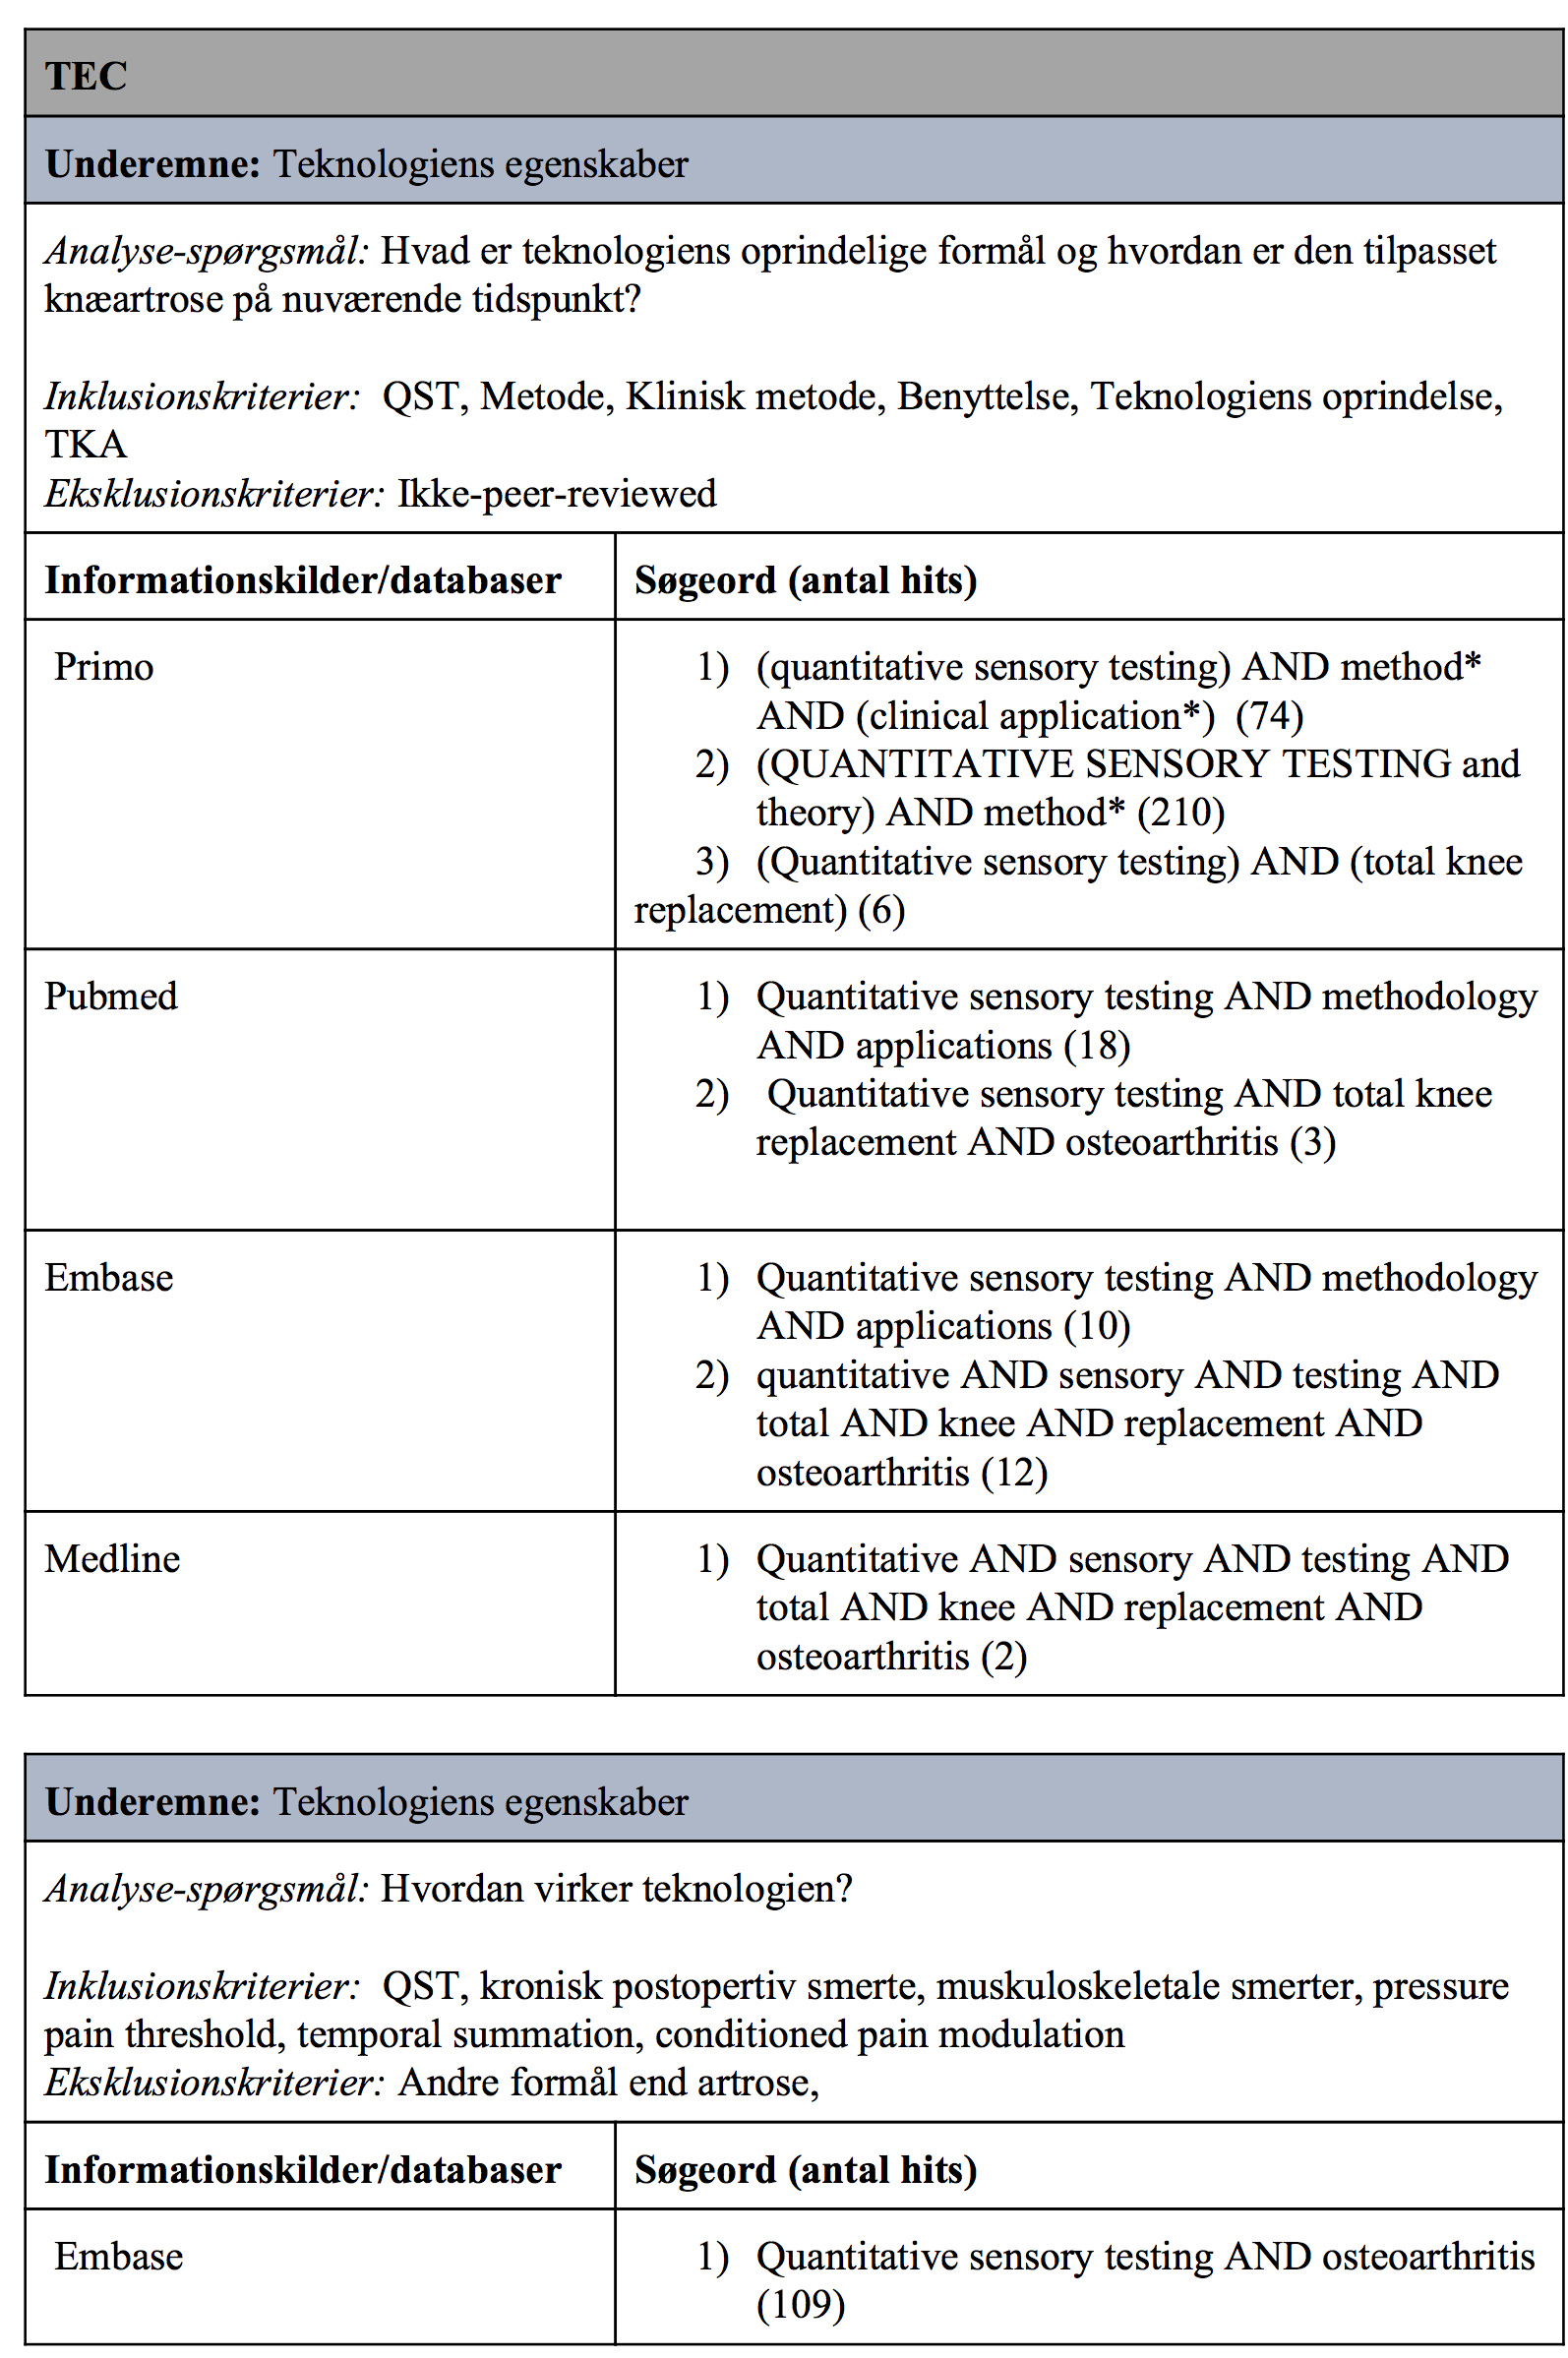
\includegraphics[width=0.8\textwidth]{rapportAfsnit/qBilag/sogninger/TEC1}

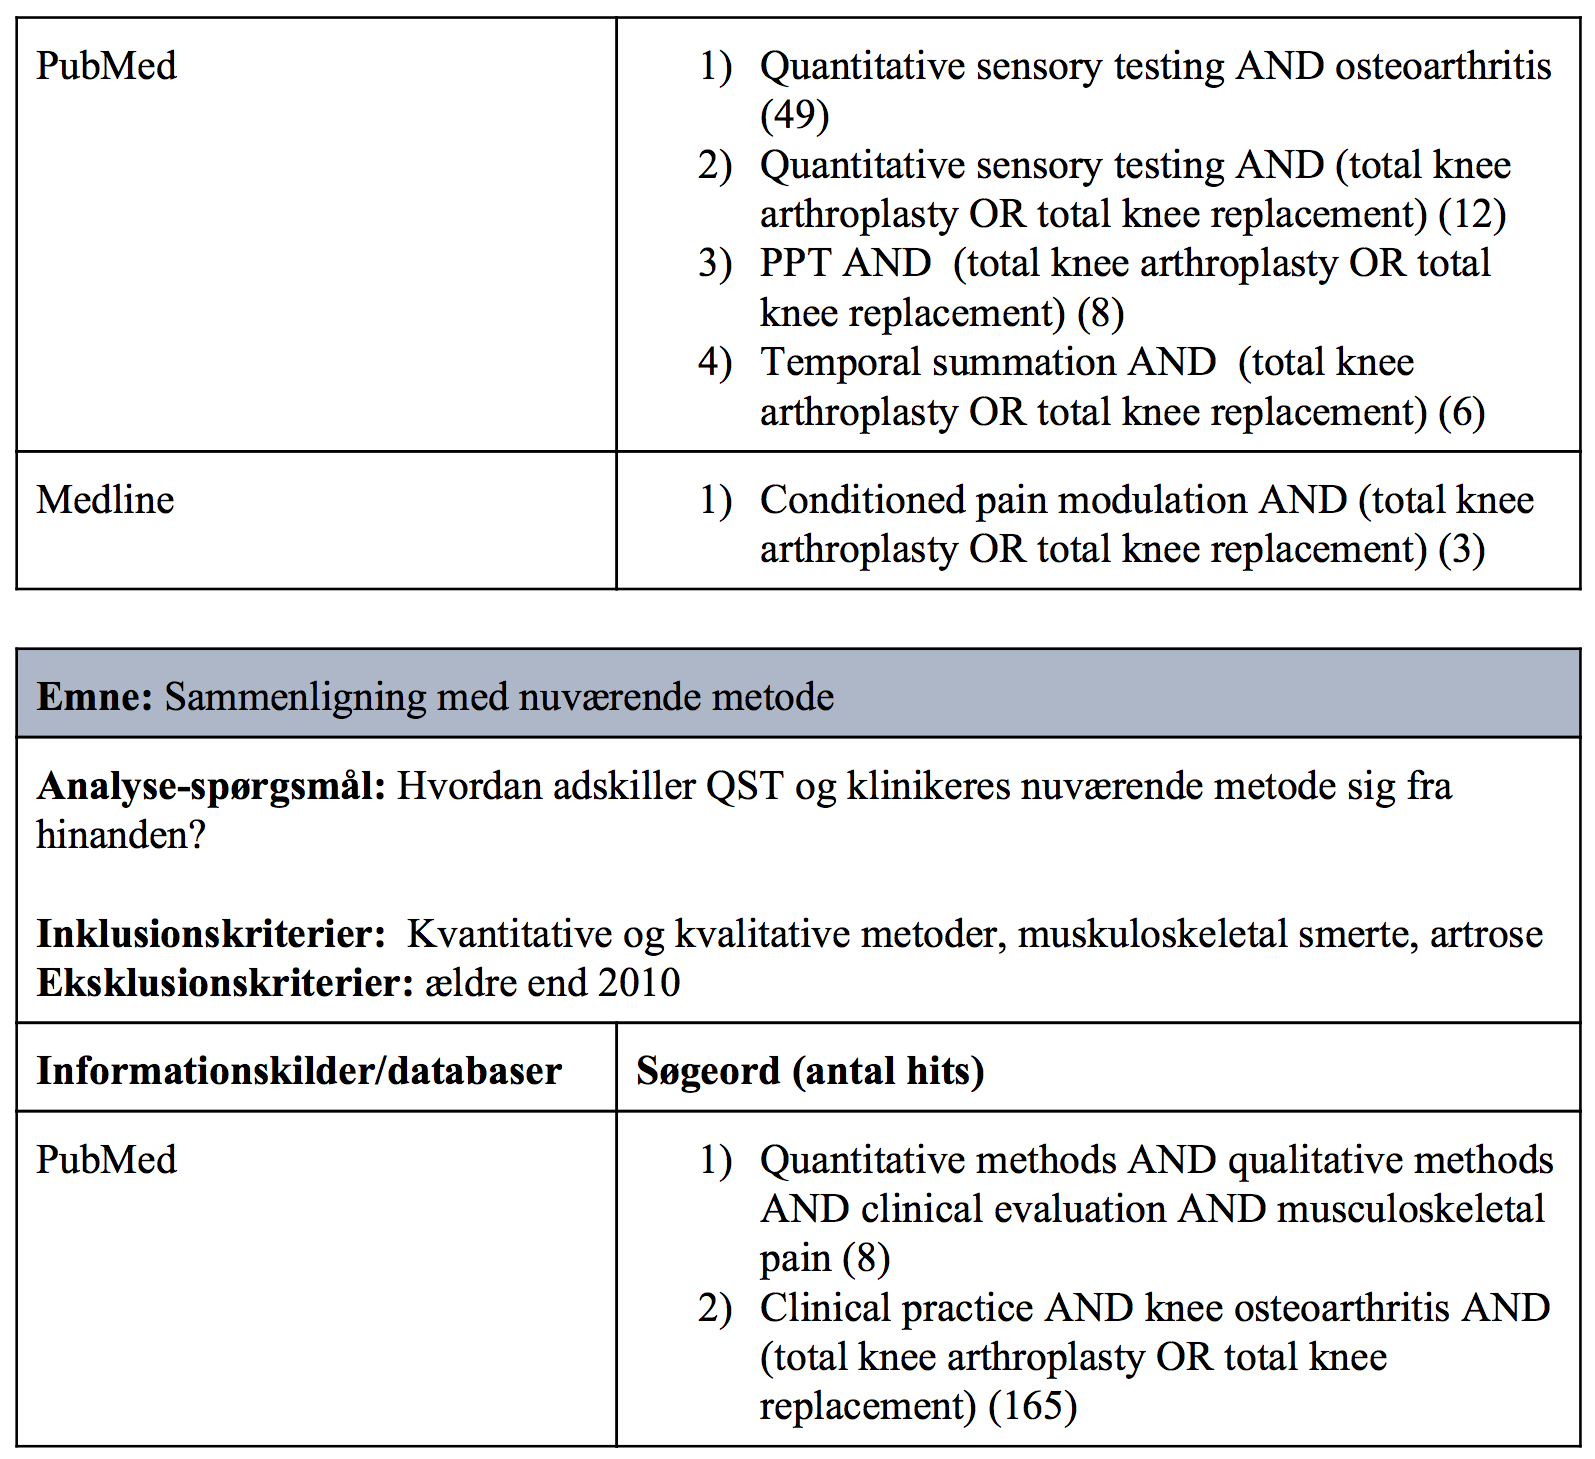
\includegraphics[width=0.8\textwidth]{rapportAfsnit/qBilag/sogninger/TEC2}

\section{EFF}\label{EFF_sog}
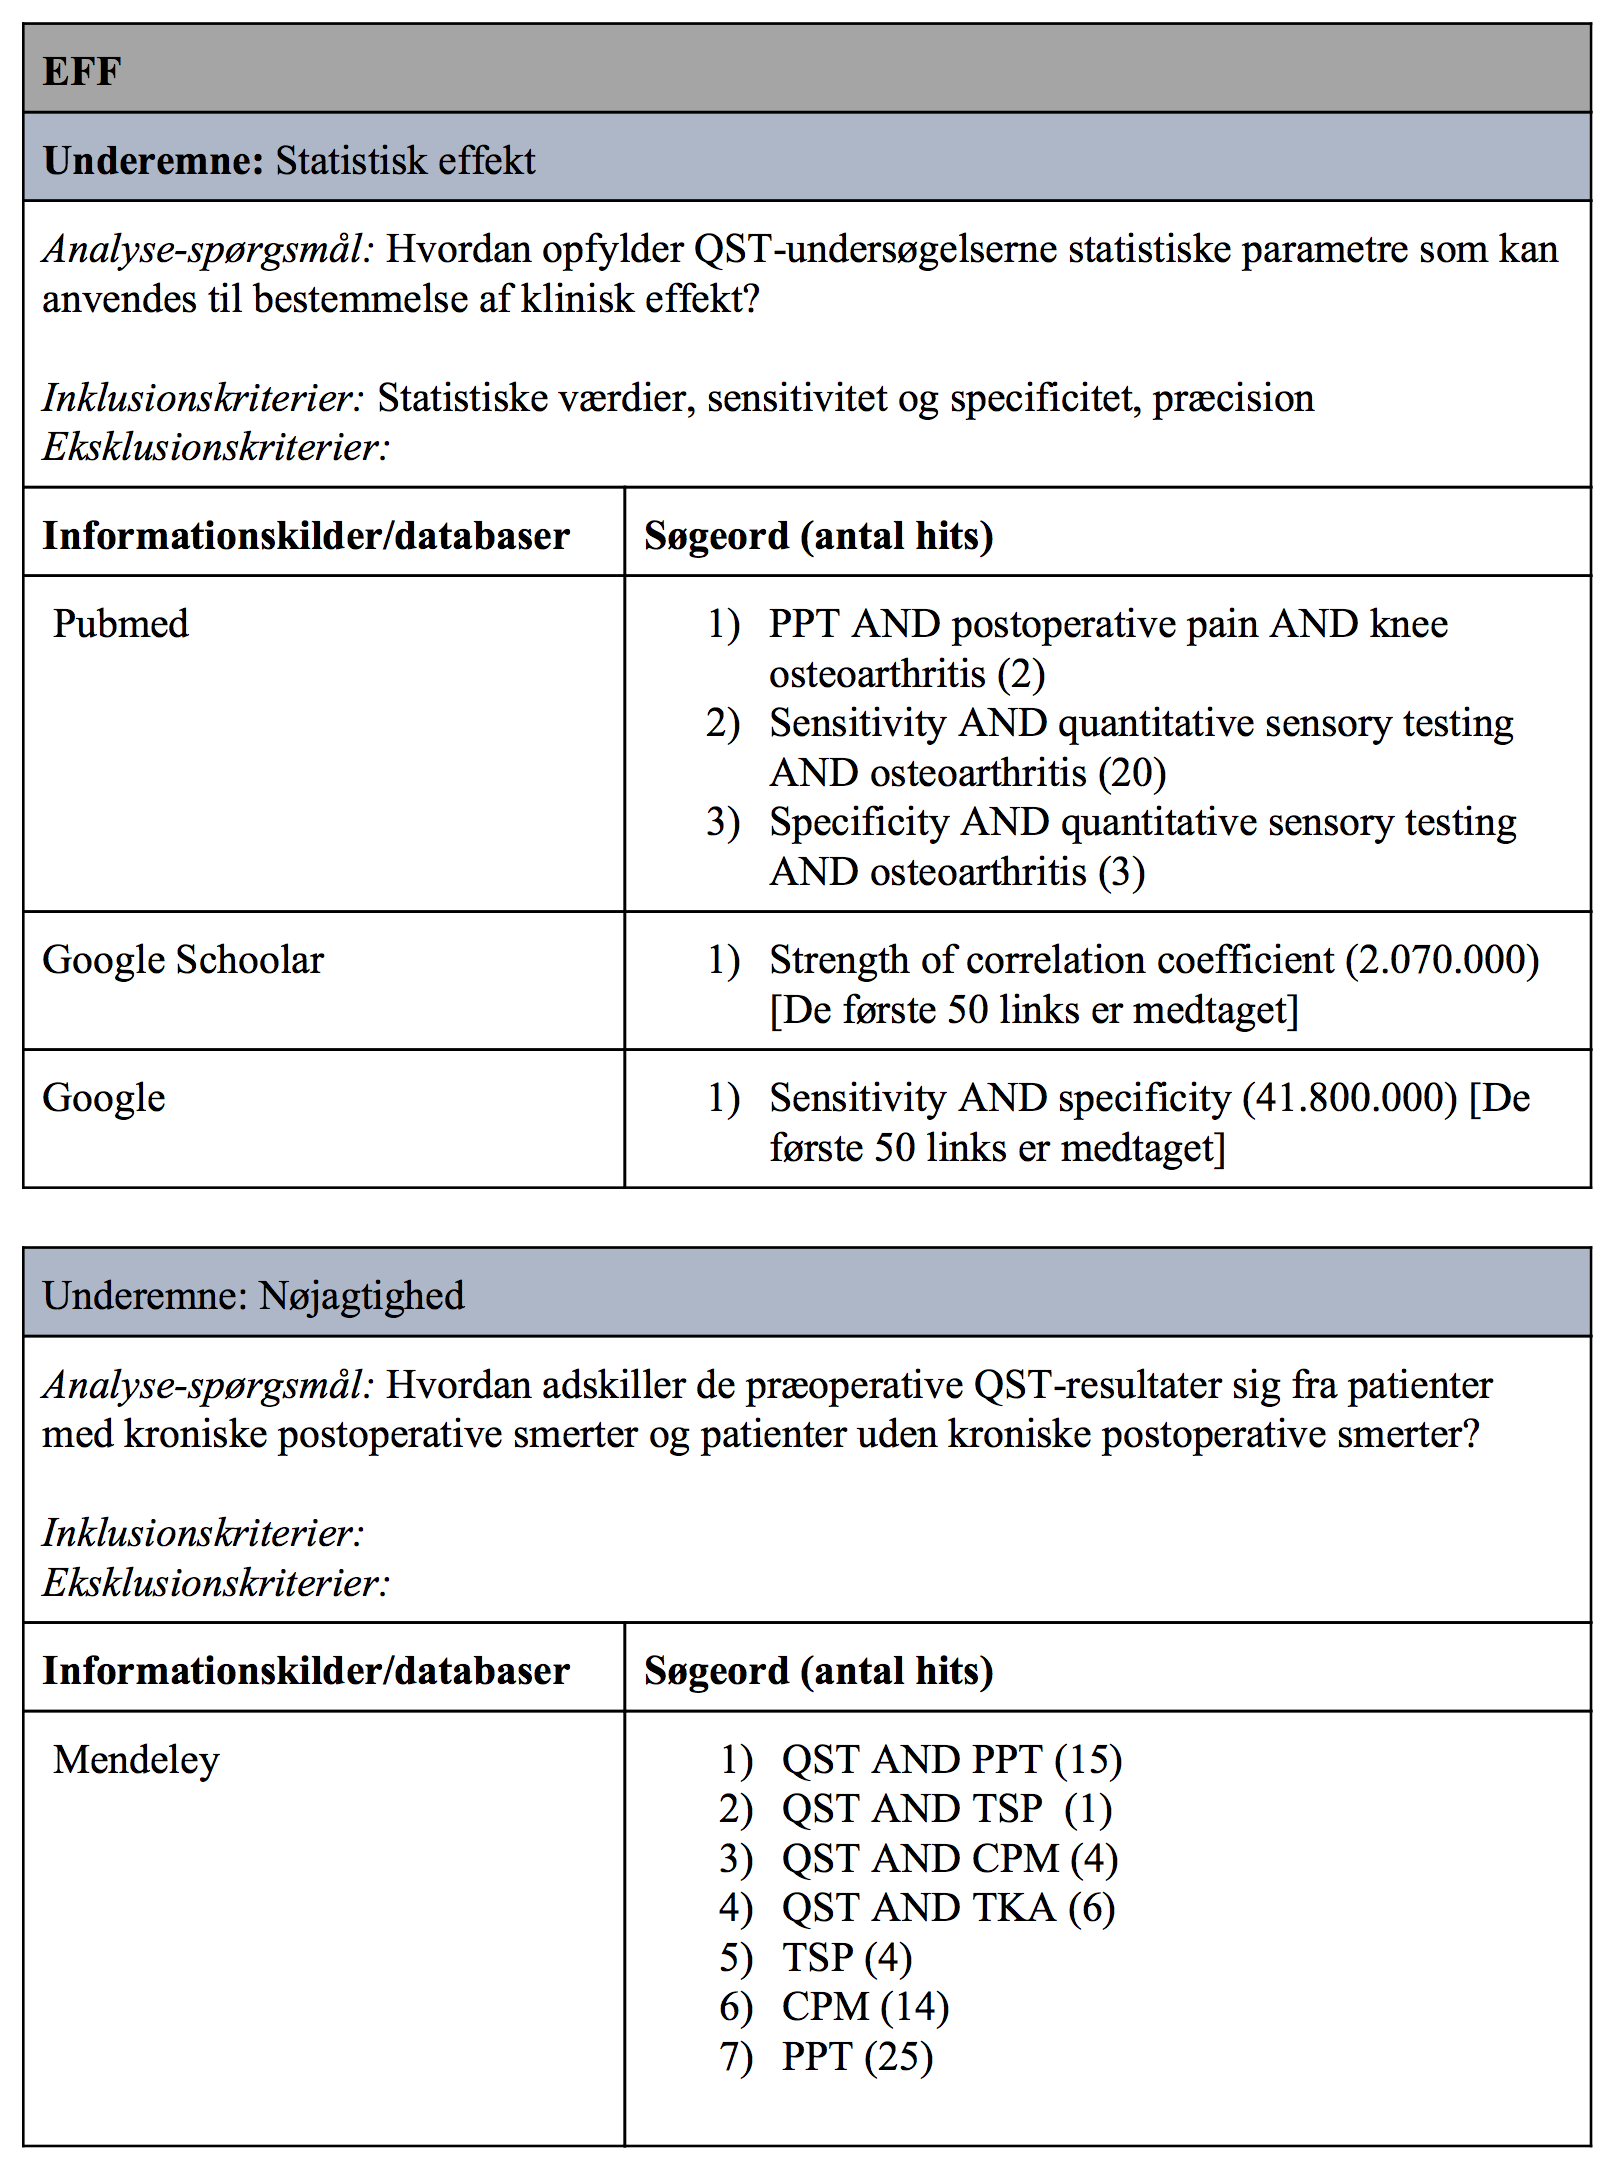
\includegraphics[width=0.8\textwidth]{rapportAfsnit/qBilag/sogninger/EFF1}

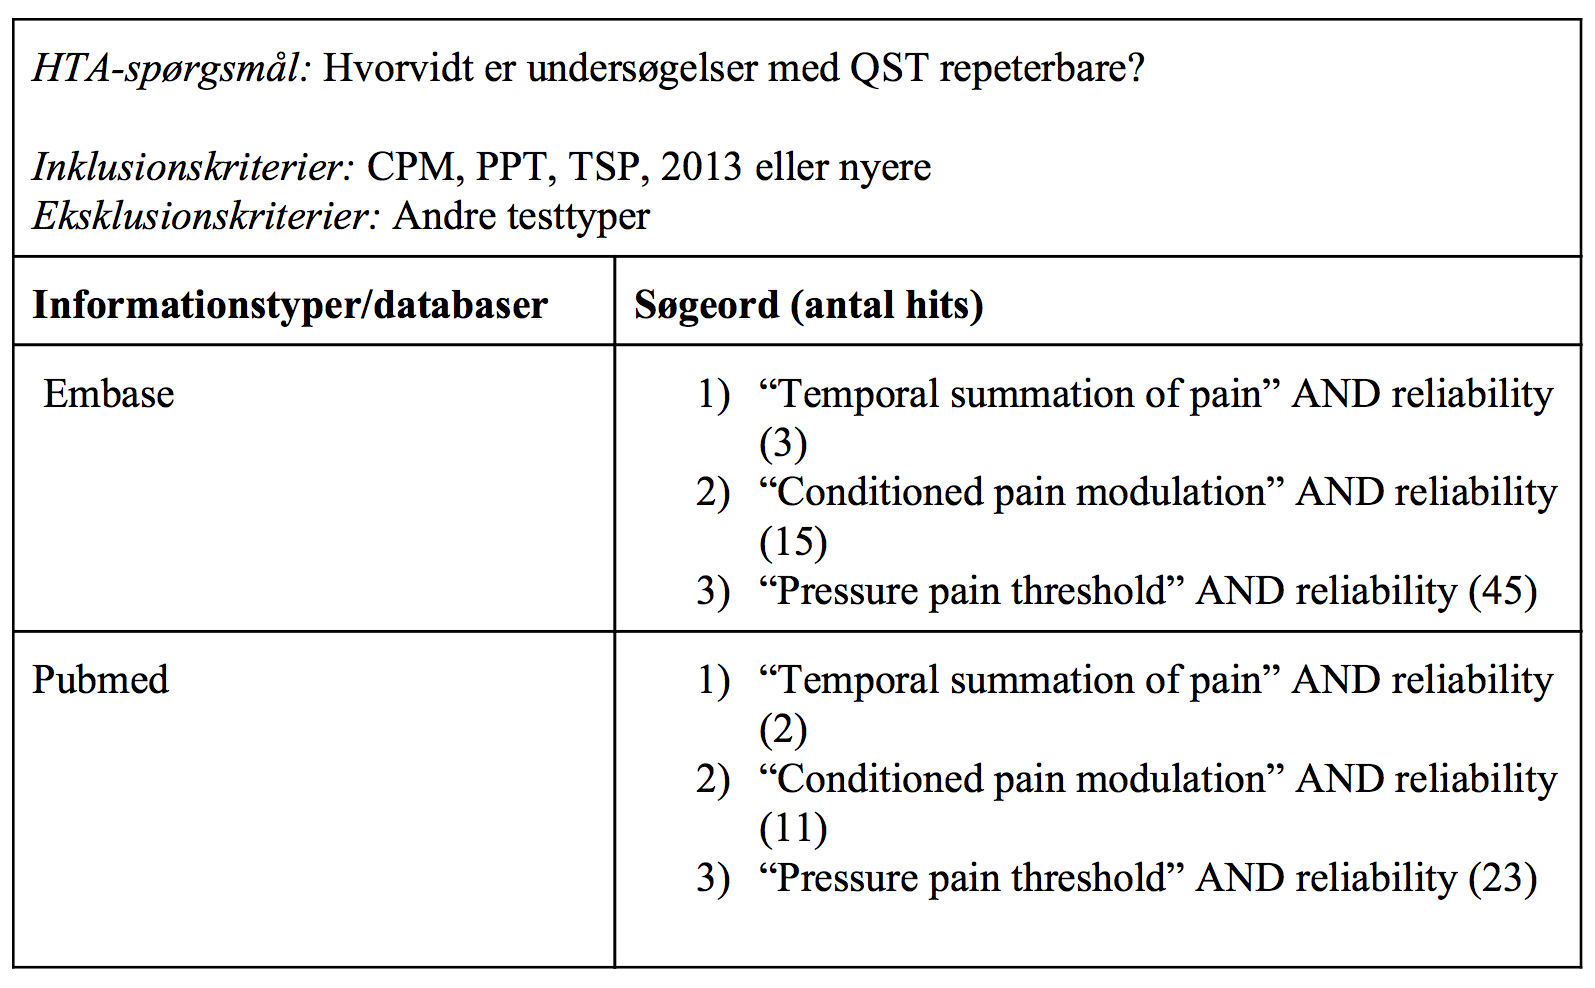
\includegraphics[width=0.8\textwidth]{rapportAfsnit/qBilag/sogninger/EFF2}

\section{SAF}\label{SAF_sog}
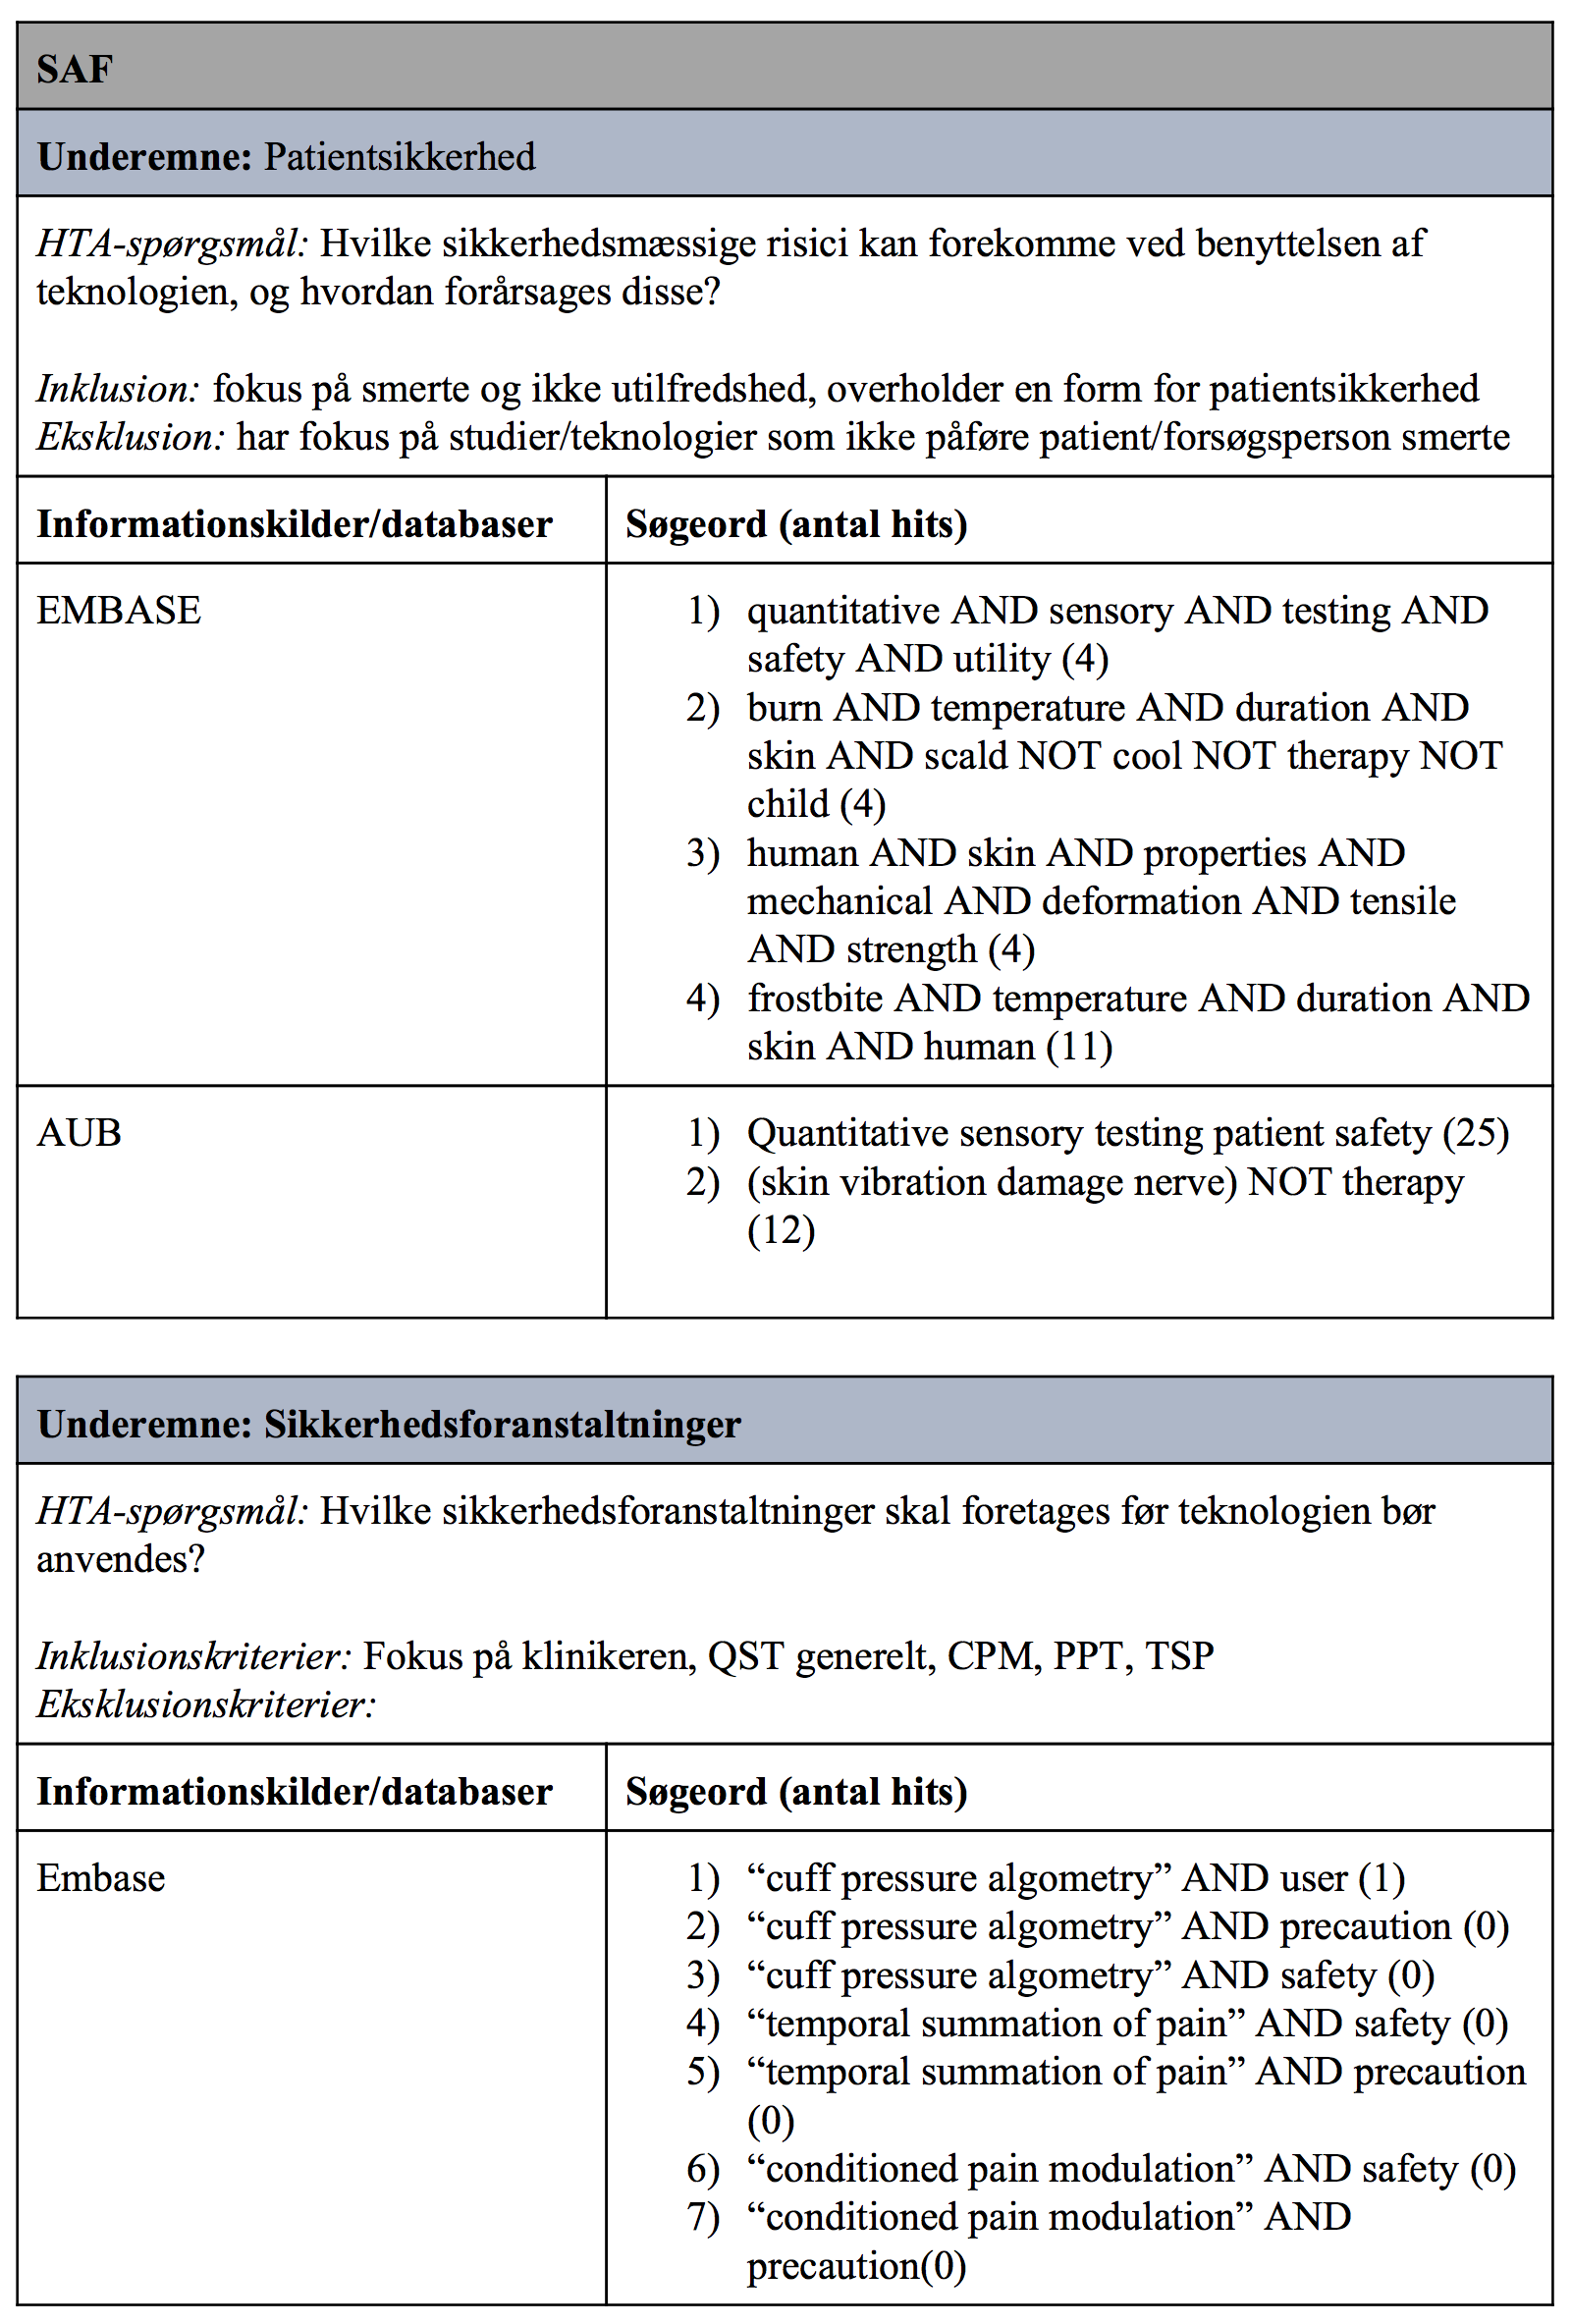
\includegraphics[width=0.8\textwidth]{rapportAfsnit/qBilag/sogninger/SAF1}

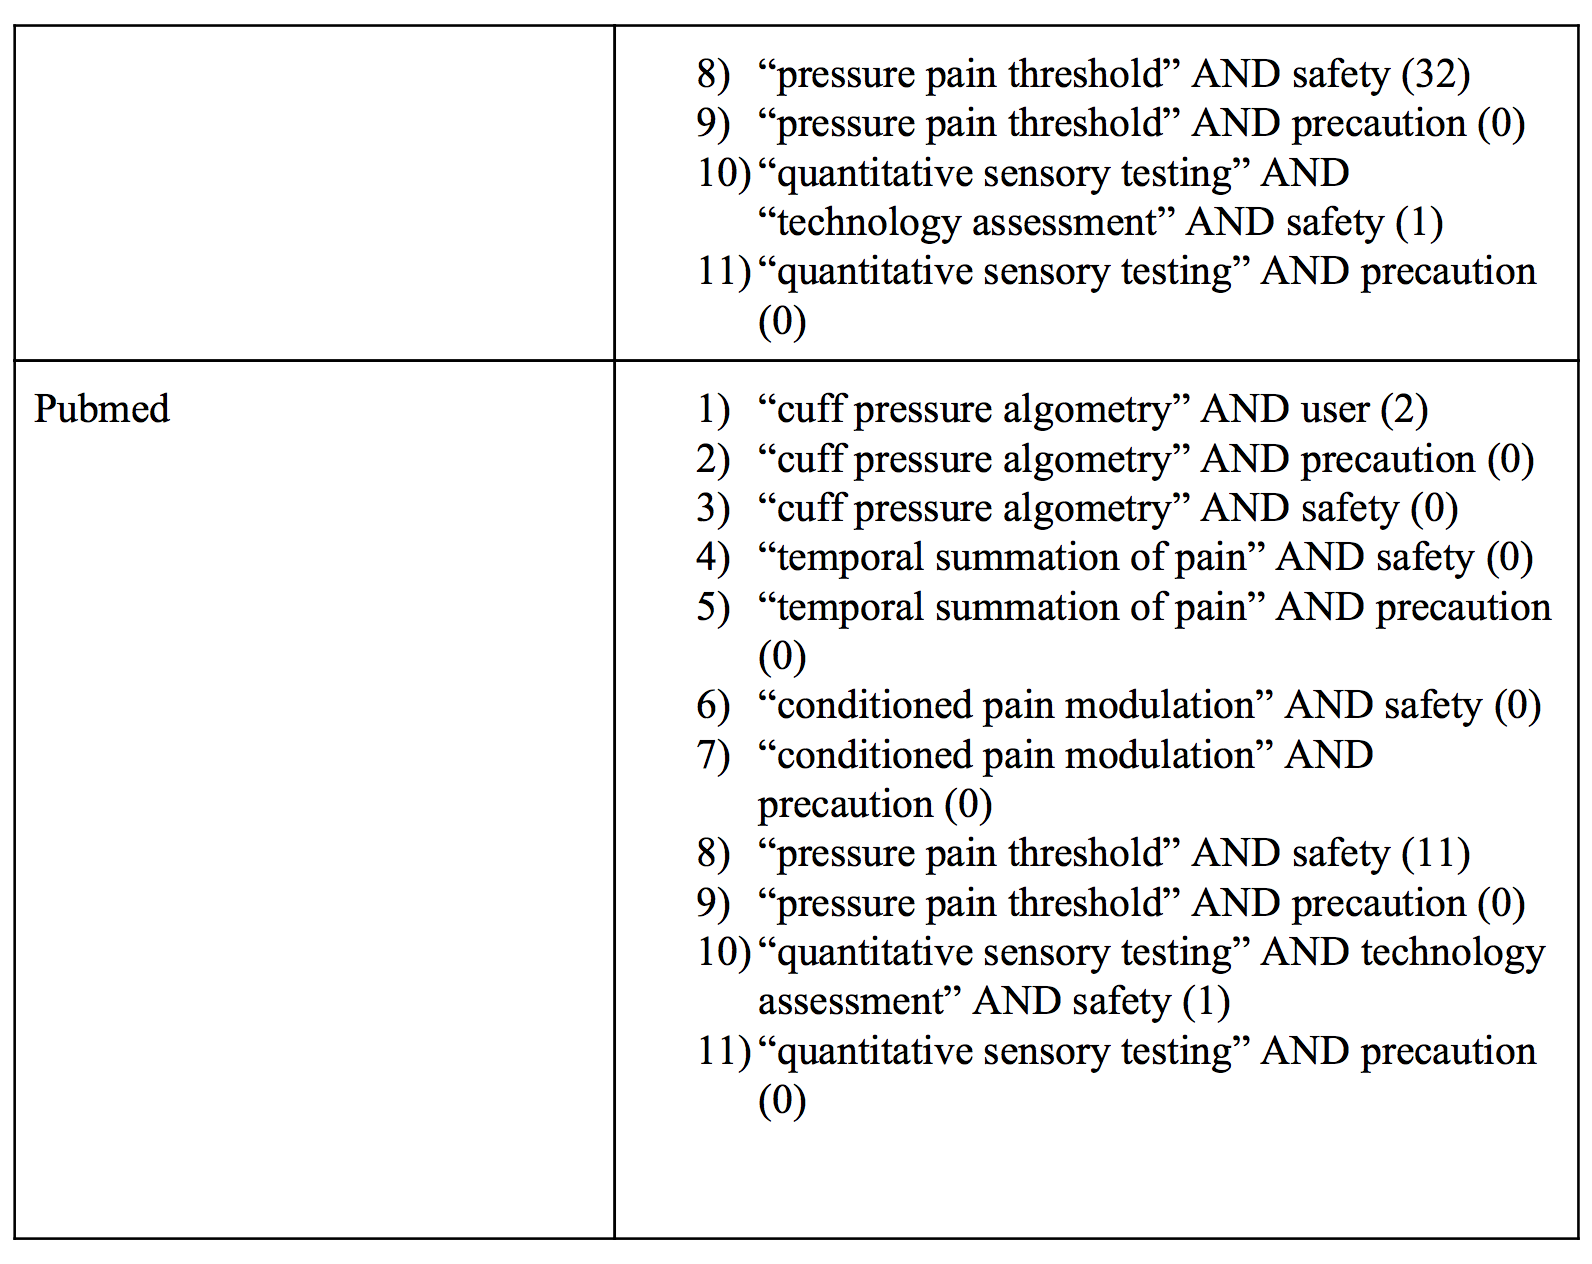
\includegraphics[width=0.8\textwidth]{rapportAfsnit/qBilag/sogninger/SAF2}

\section{ORG}\label{ORG_sog}
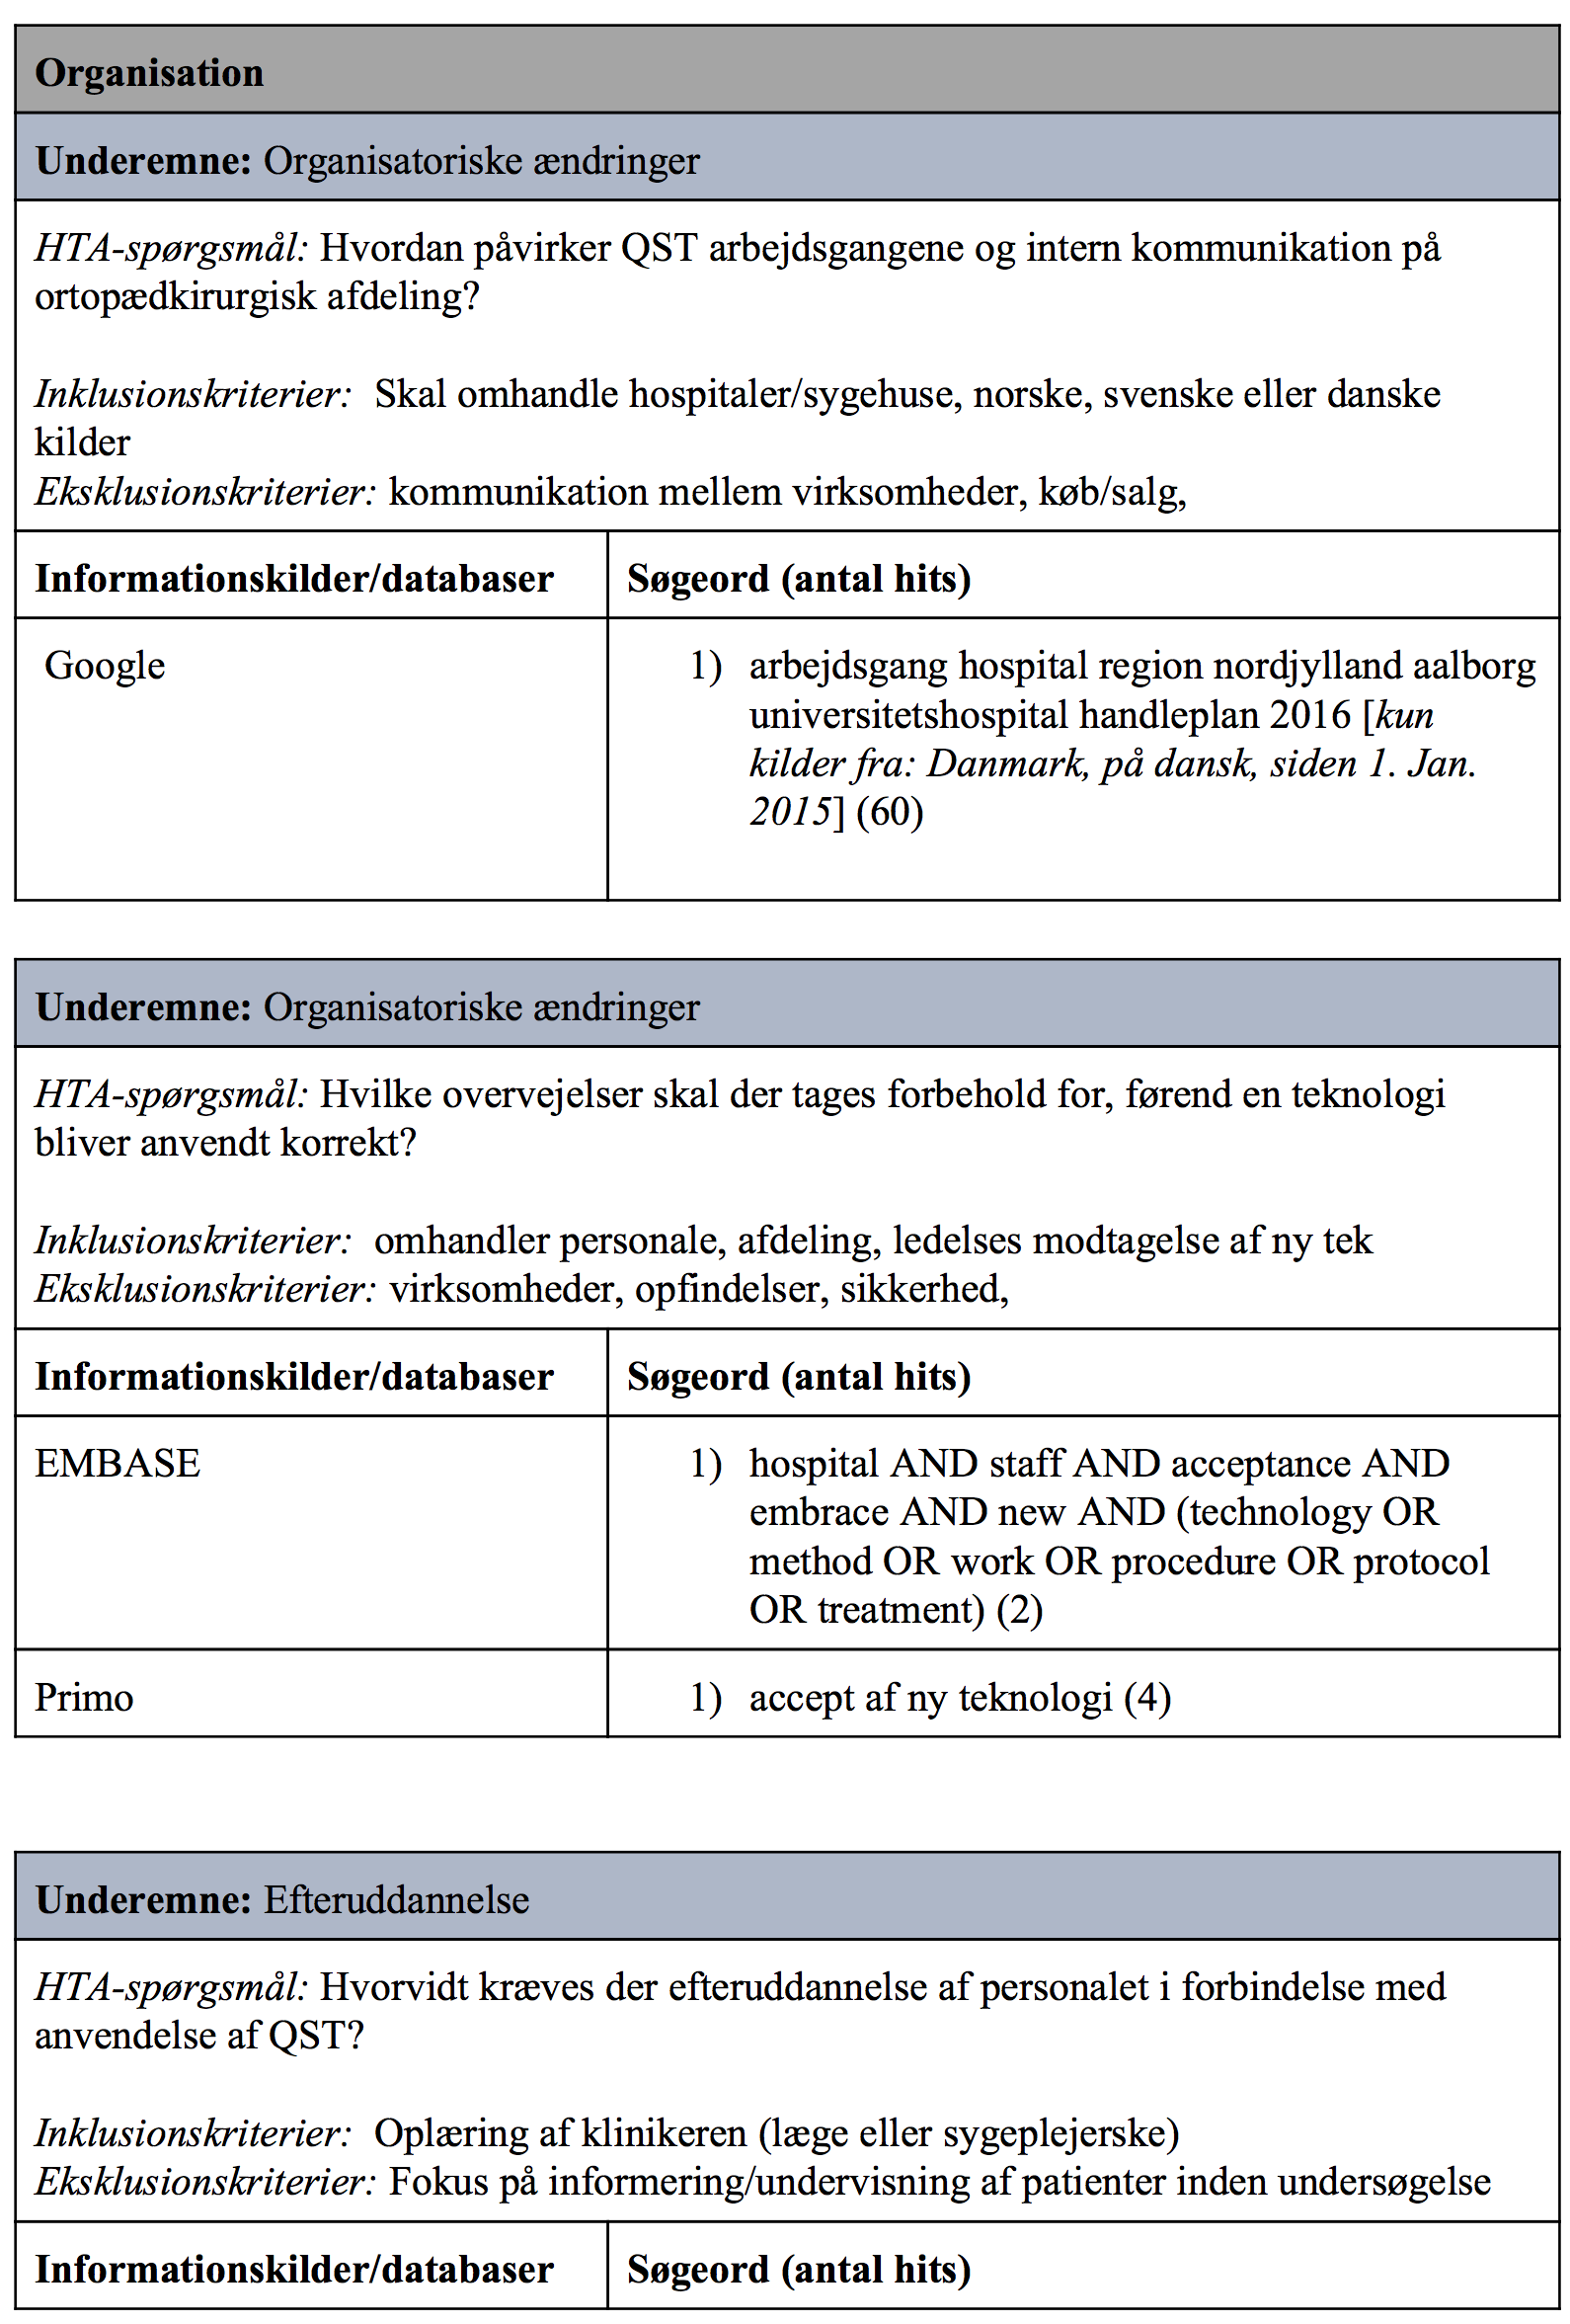
\includegraphics[width=0.8\textwidth]{rapportAfsnit/qBilag/sogninger/ORG1}

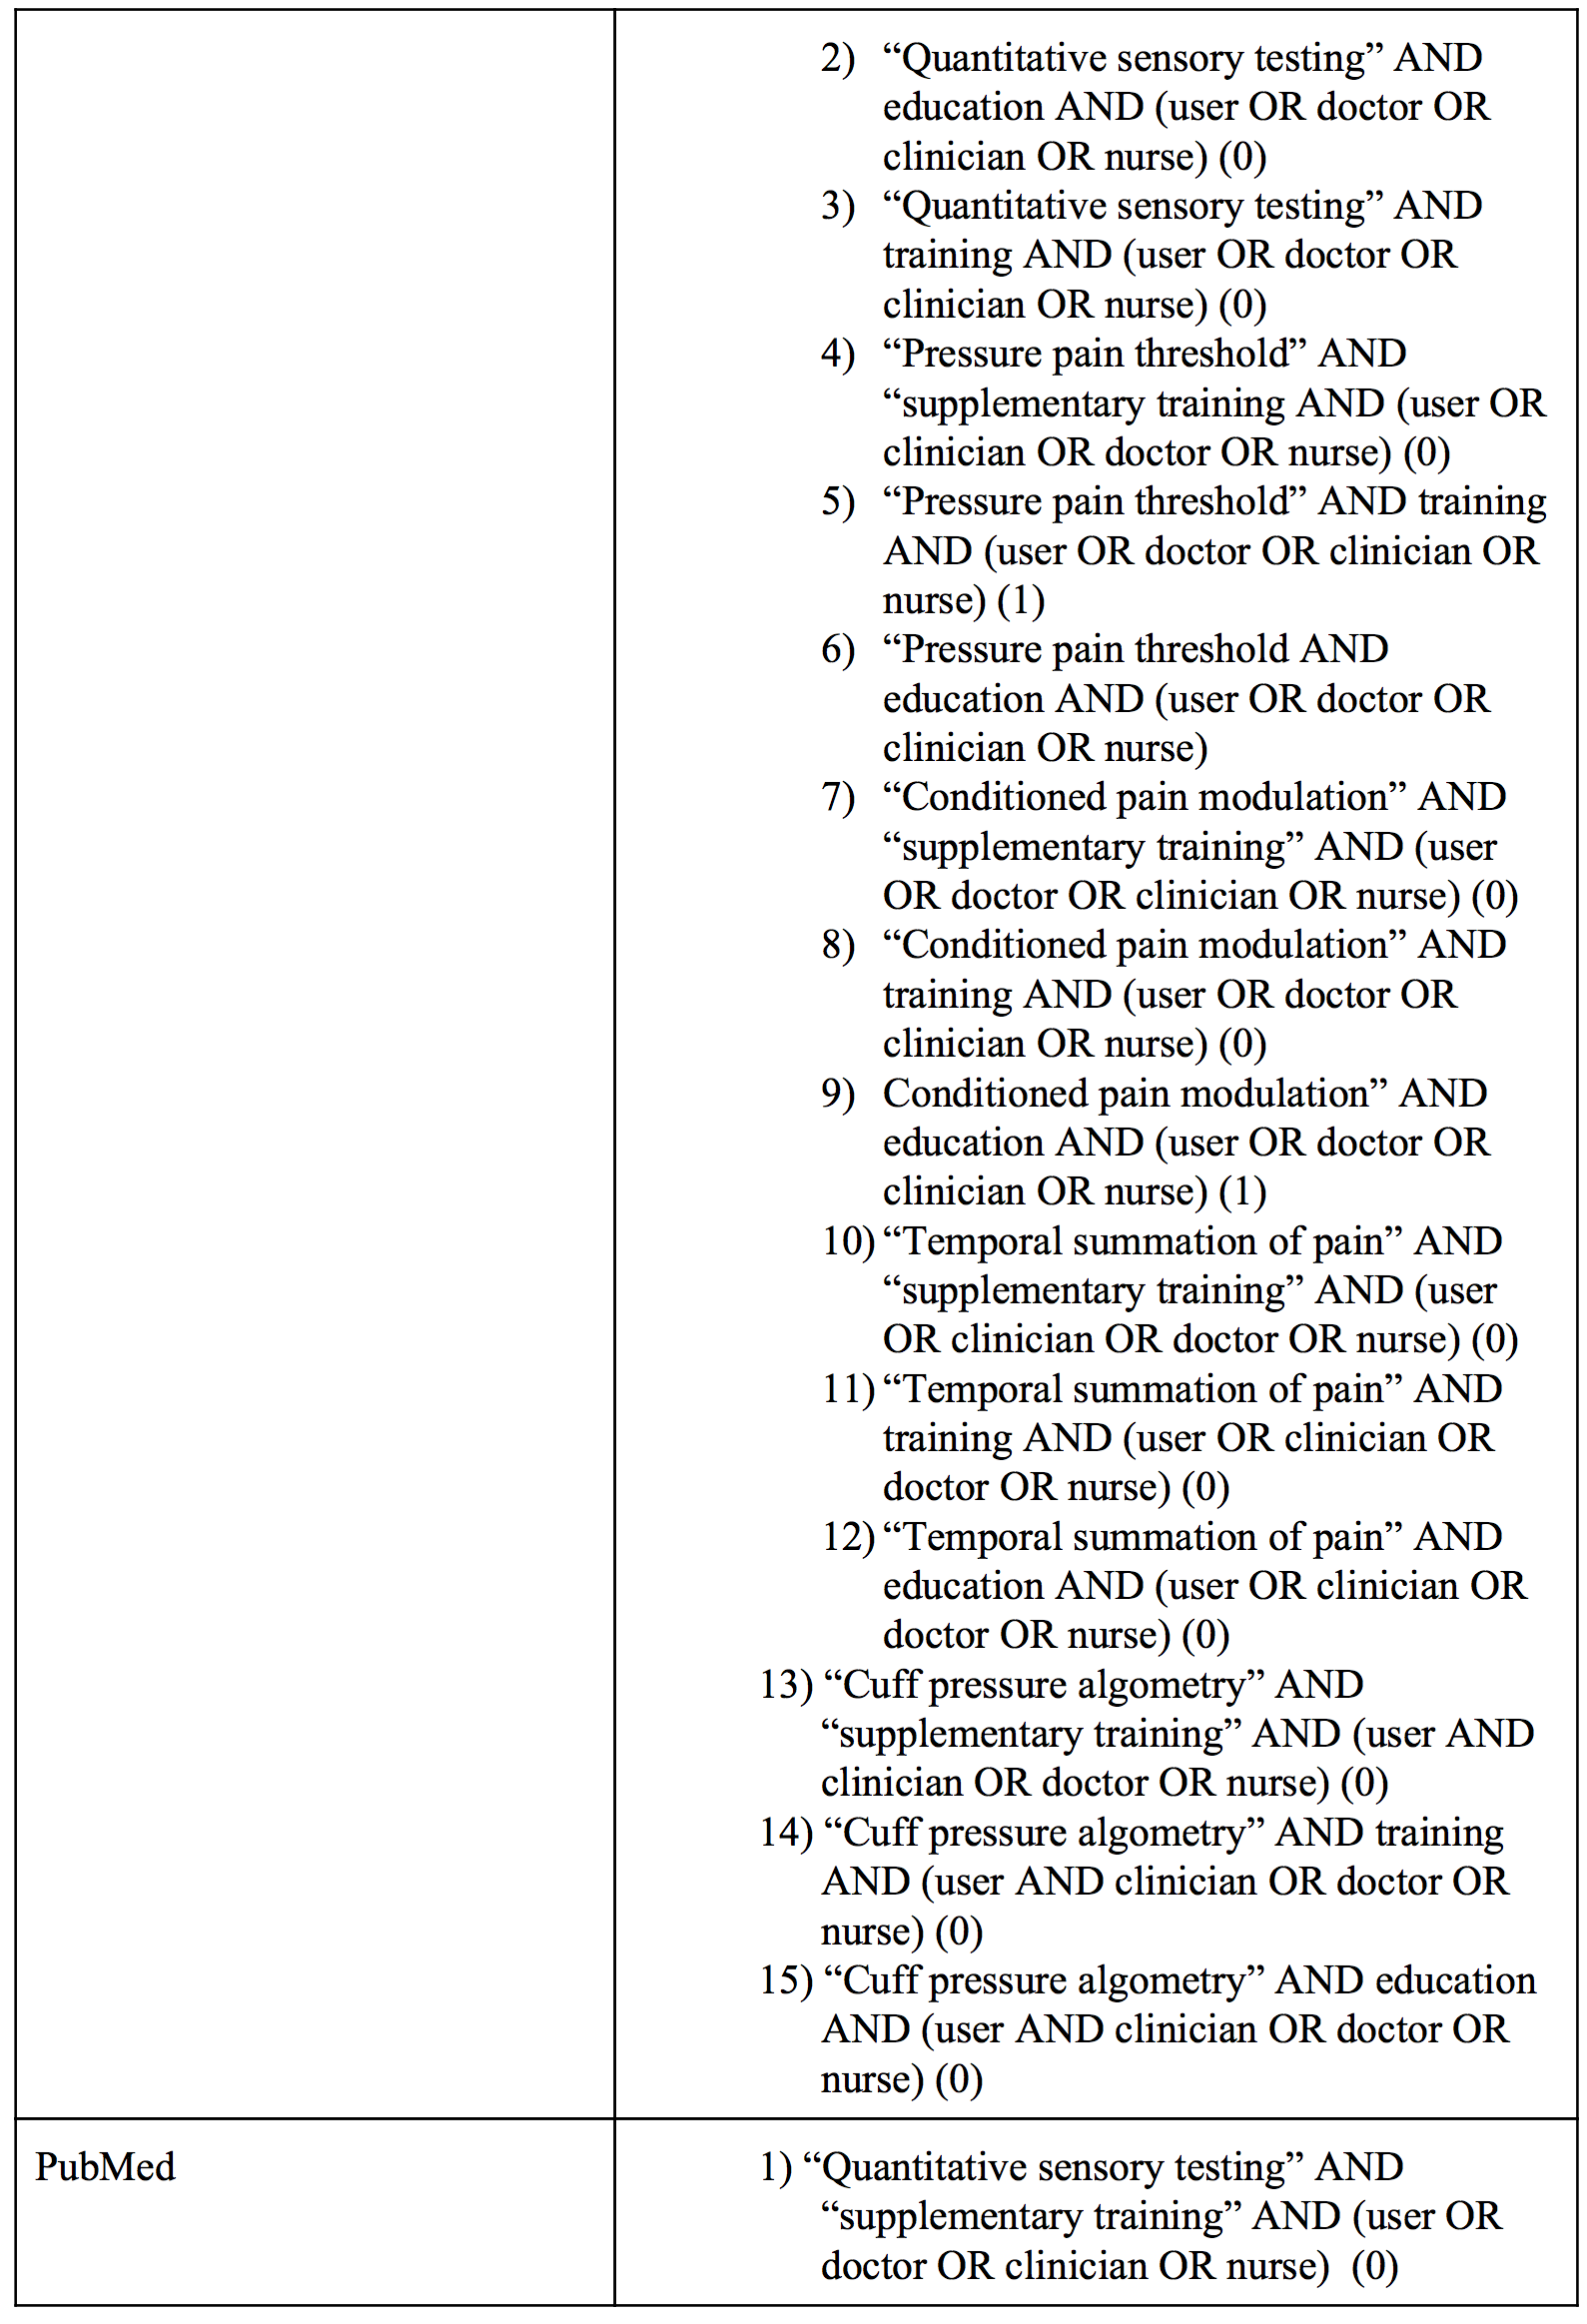
\includegraphics[width=0.8\textwidth]{rapportAfsnit/qBilag/sogninger/ORG2}

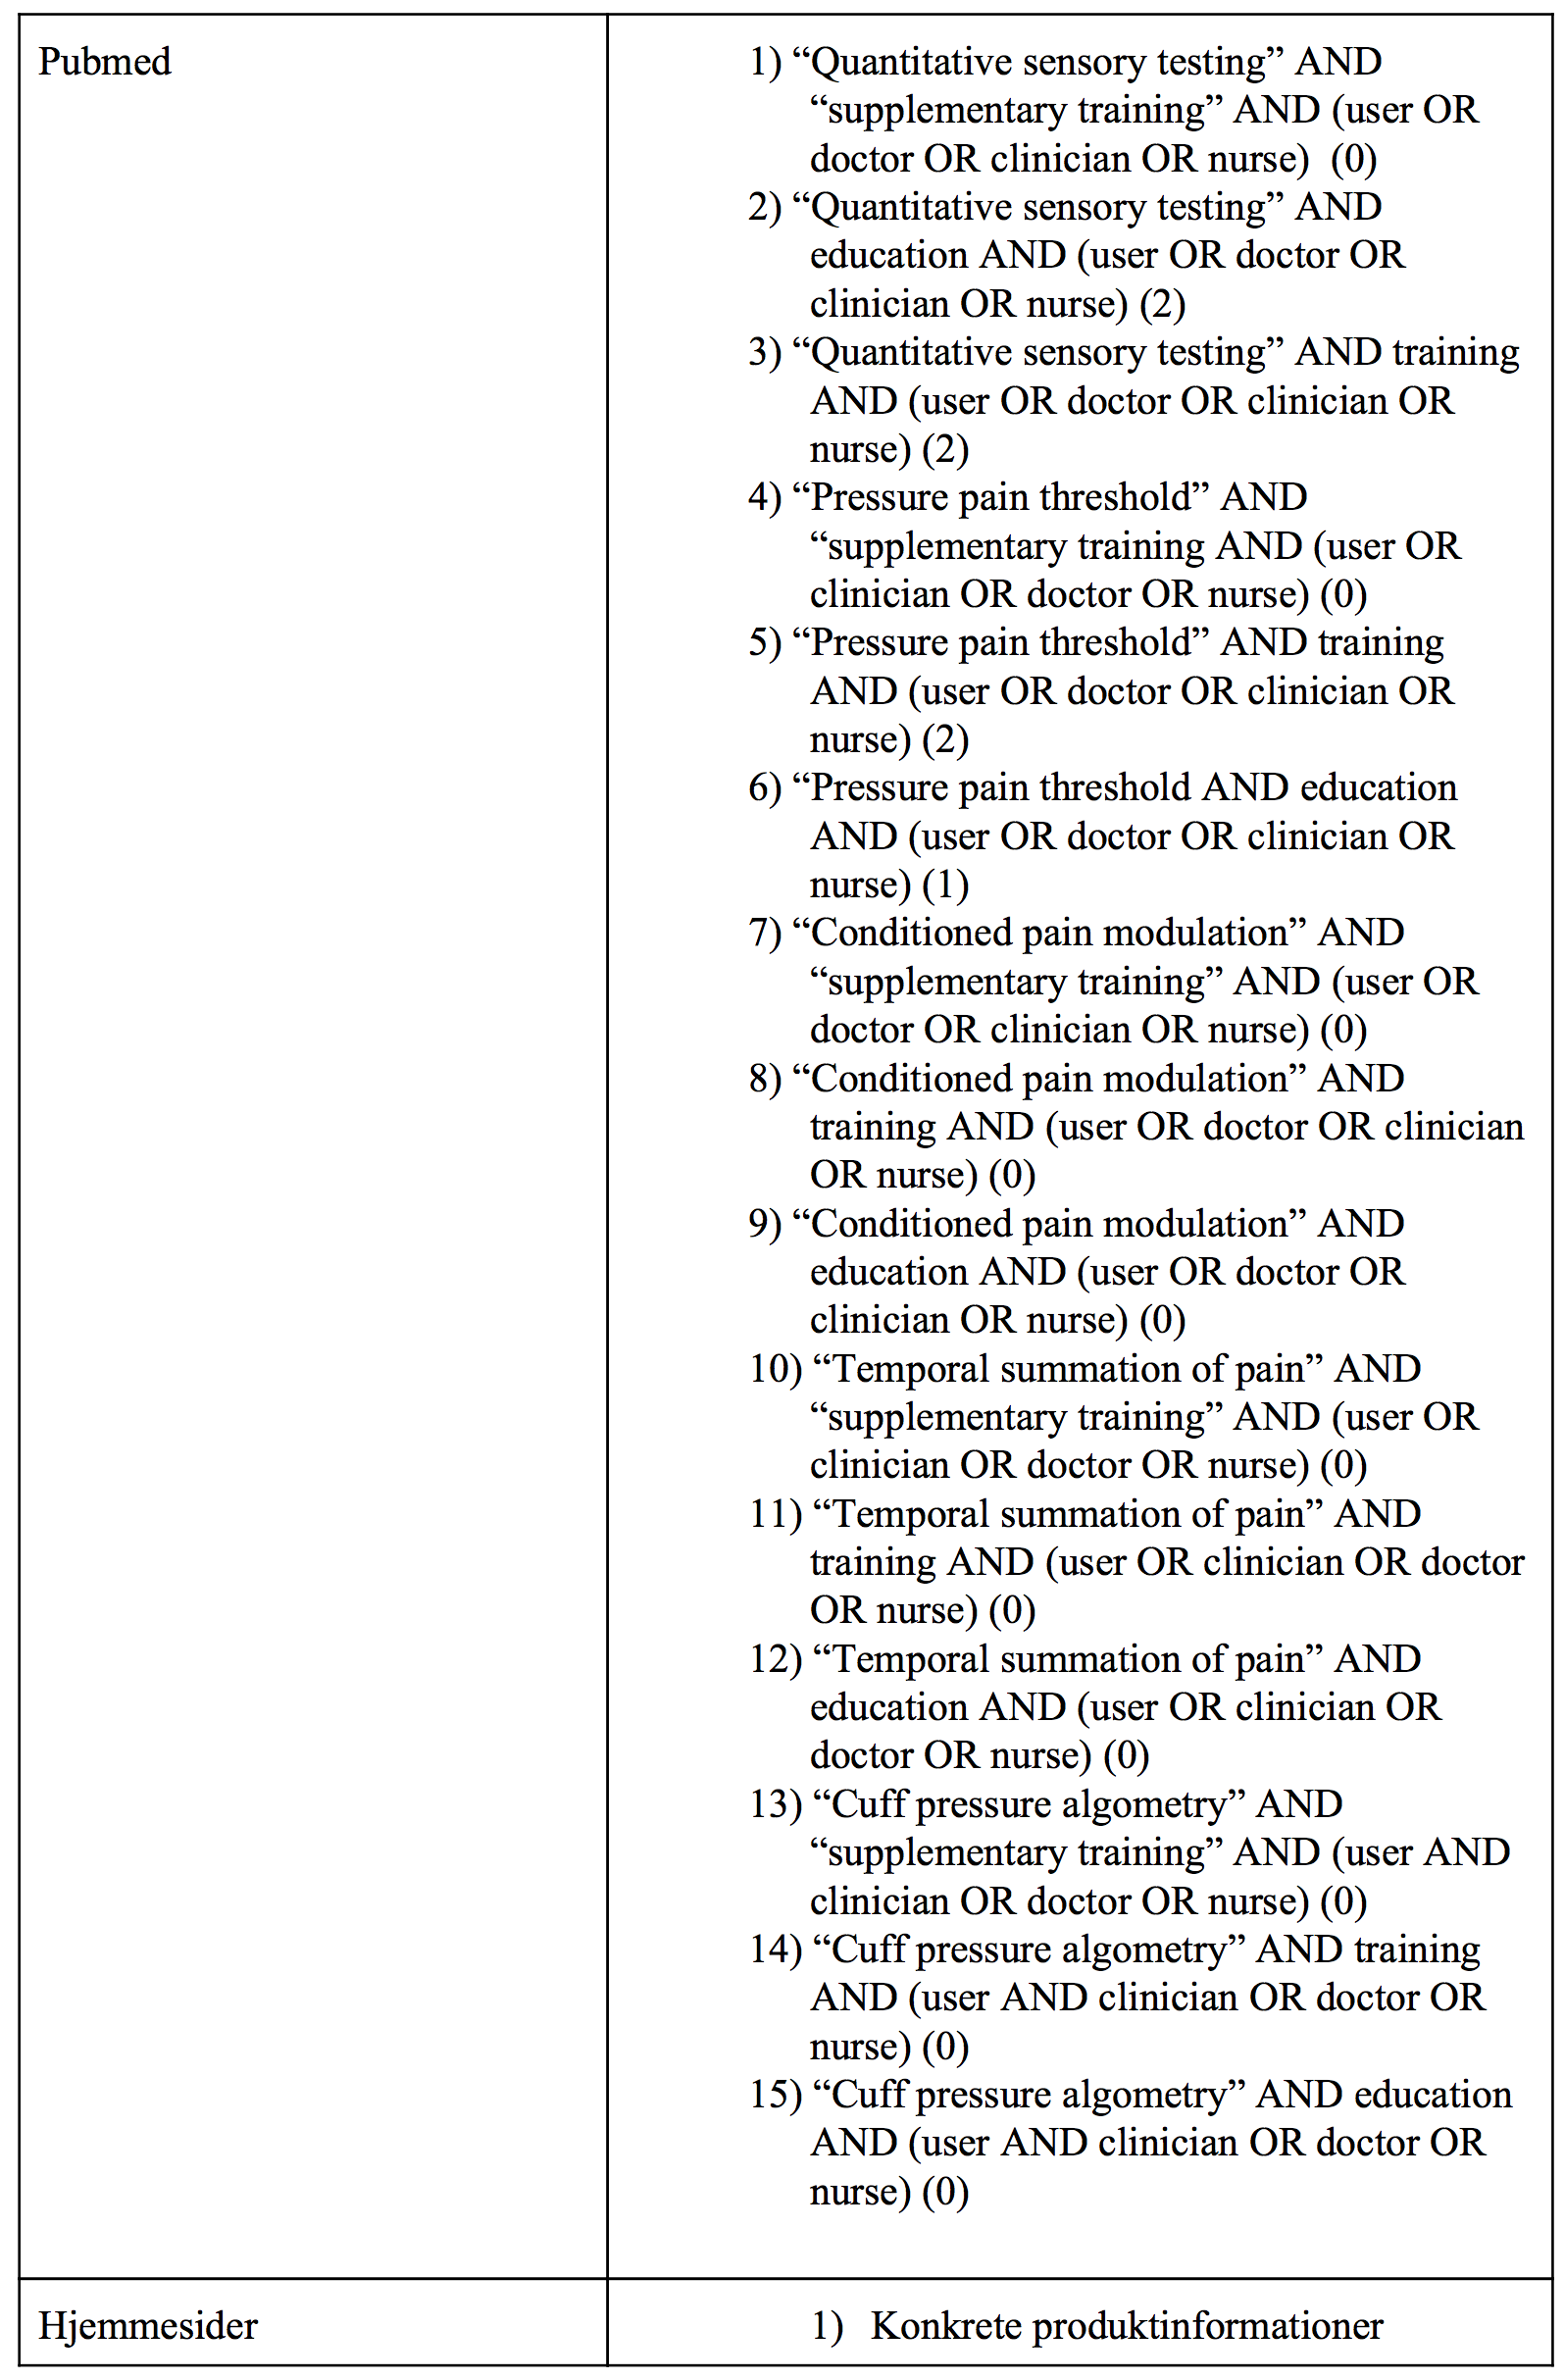
\includegraphics[width=0.8\textwidth]{rapportAfsnit/qBilag/sogninger/ORG3}

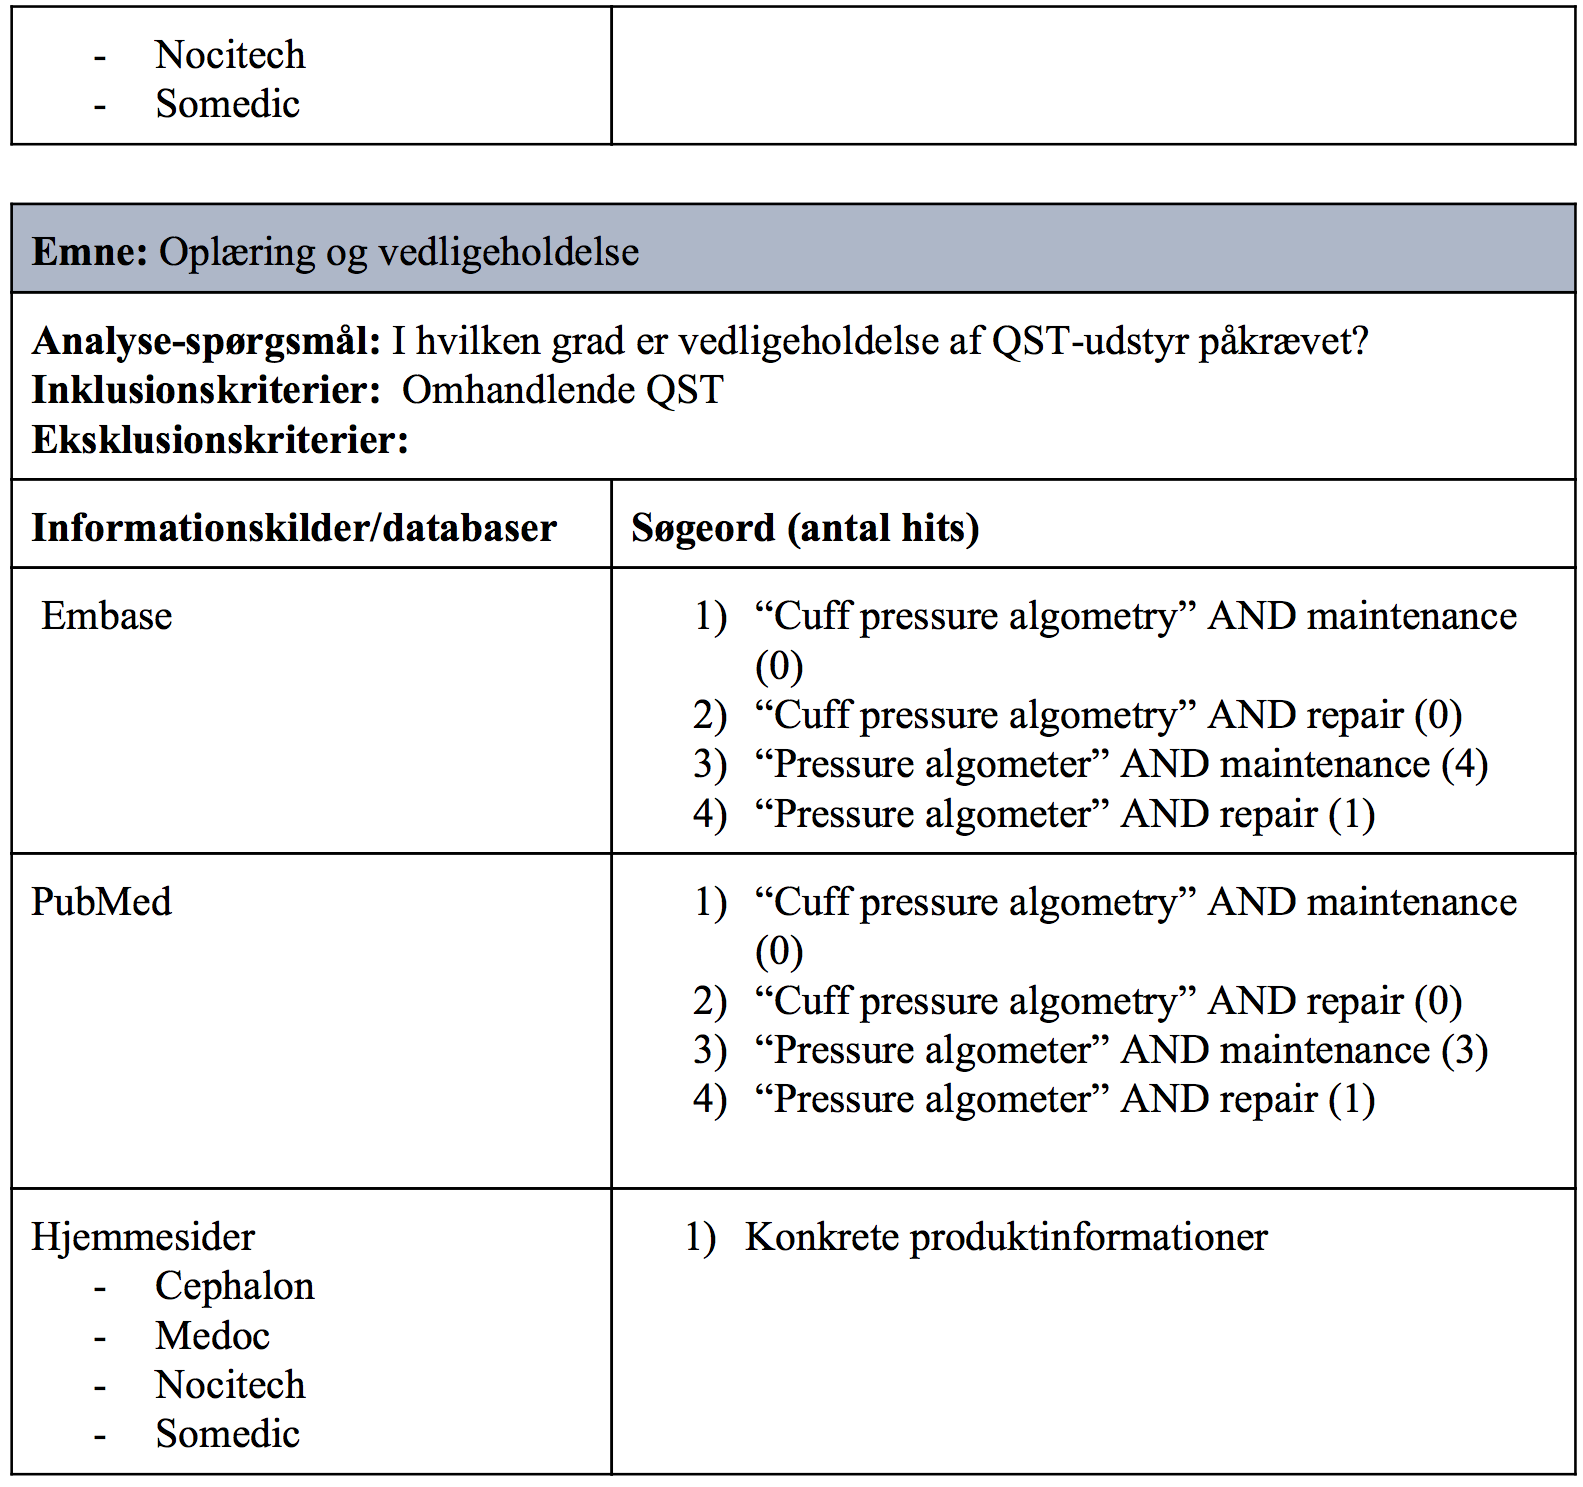
\includegraphics[width=0.8\textwidth]{rapportAfsnit/qBilag/sogninger/ORG4}

\section{SOC}\label{SOC_sog}
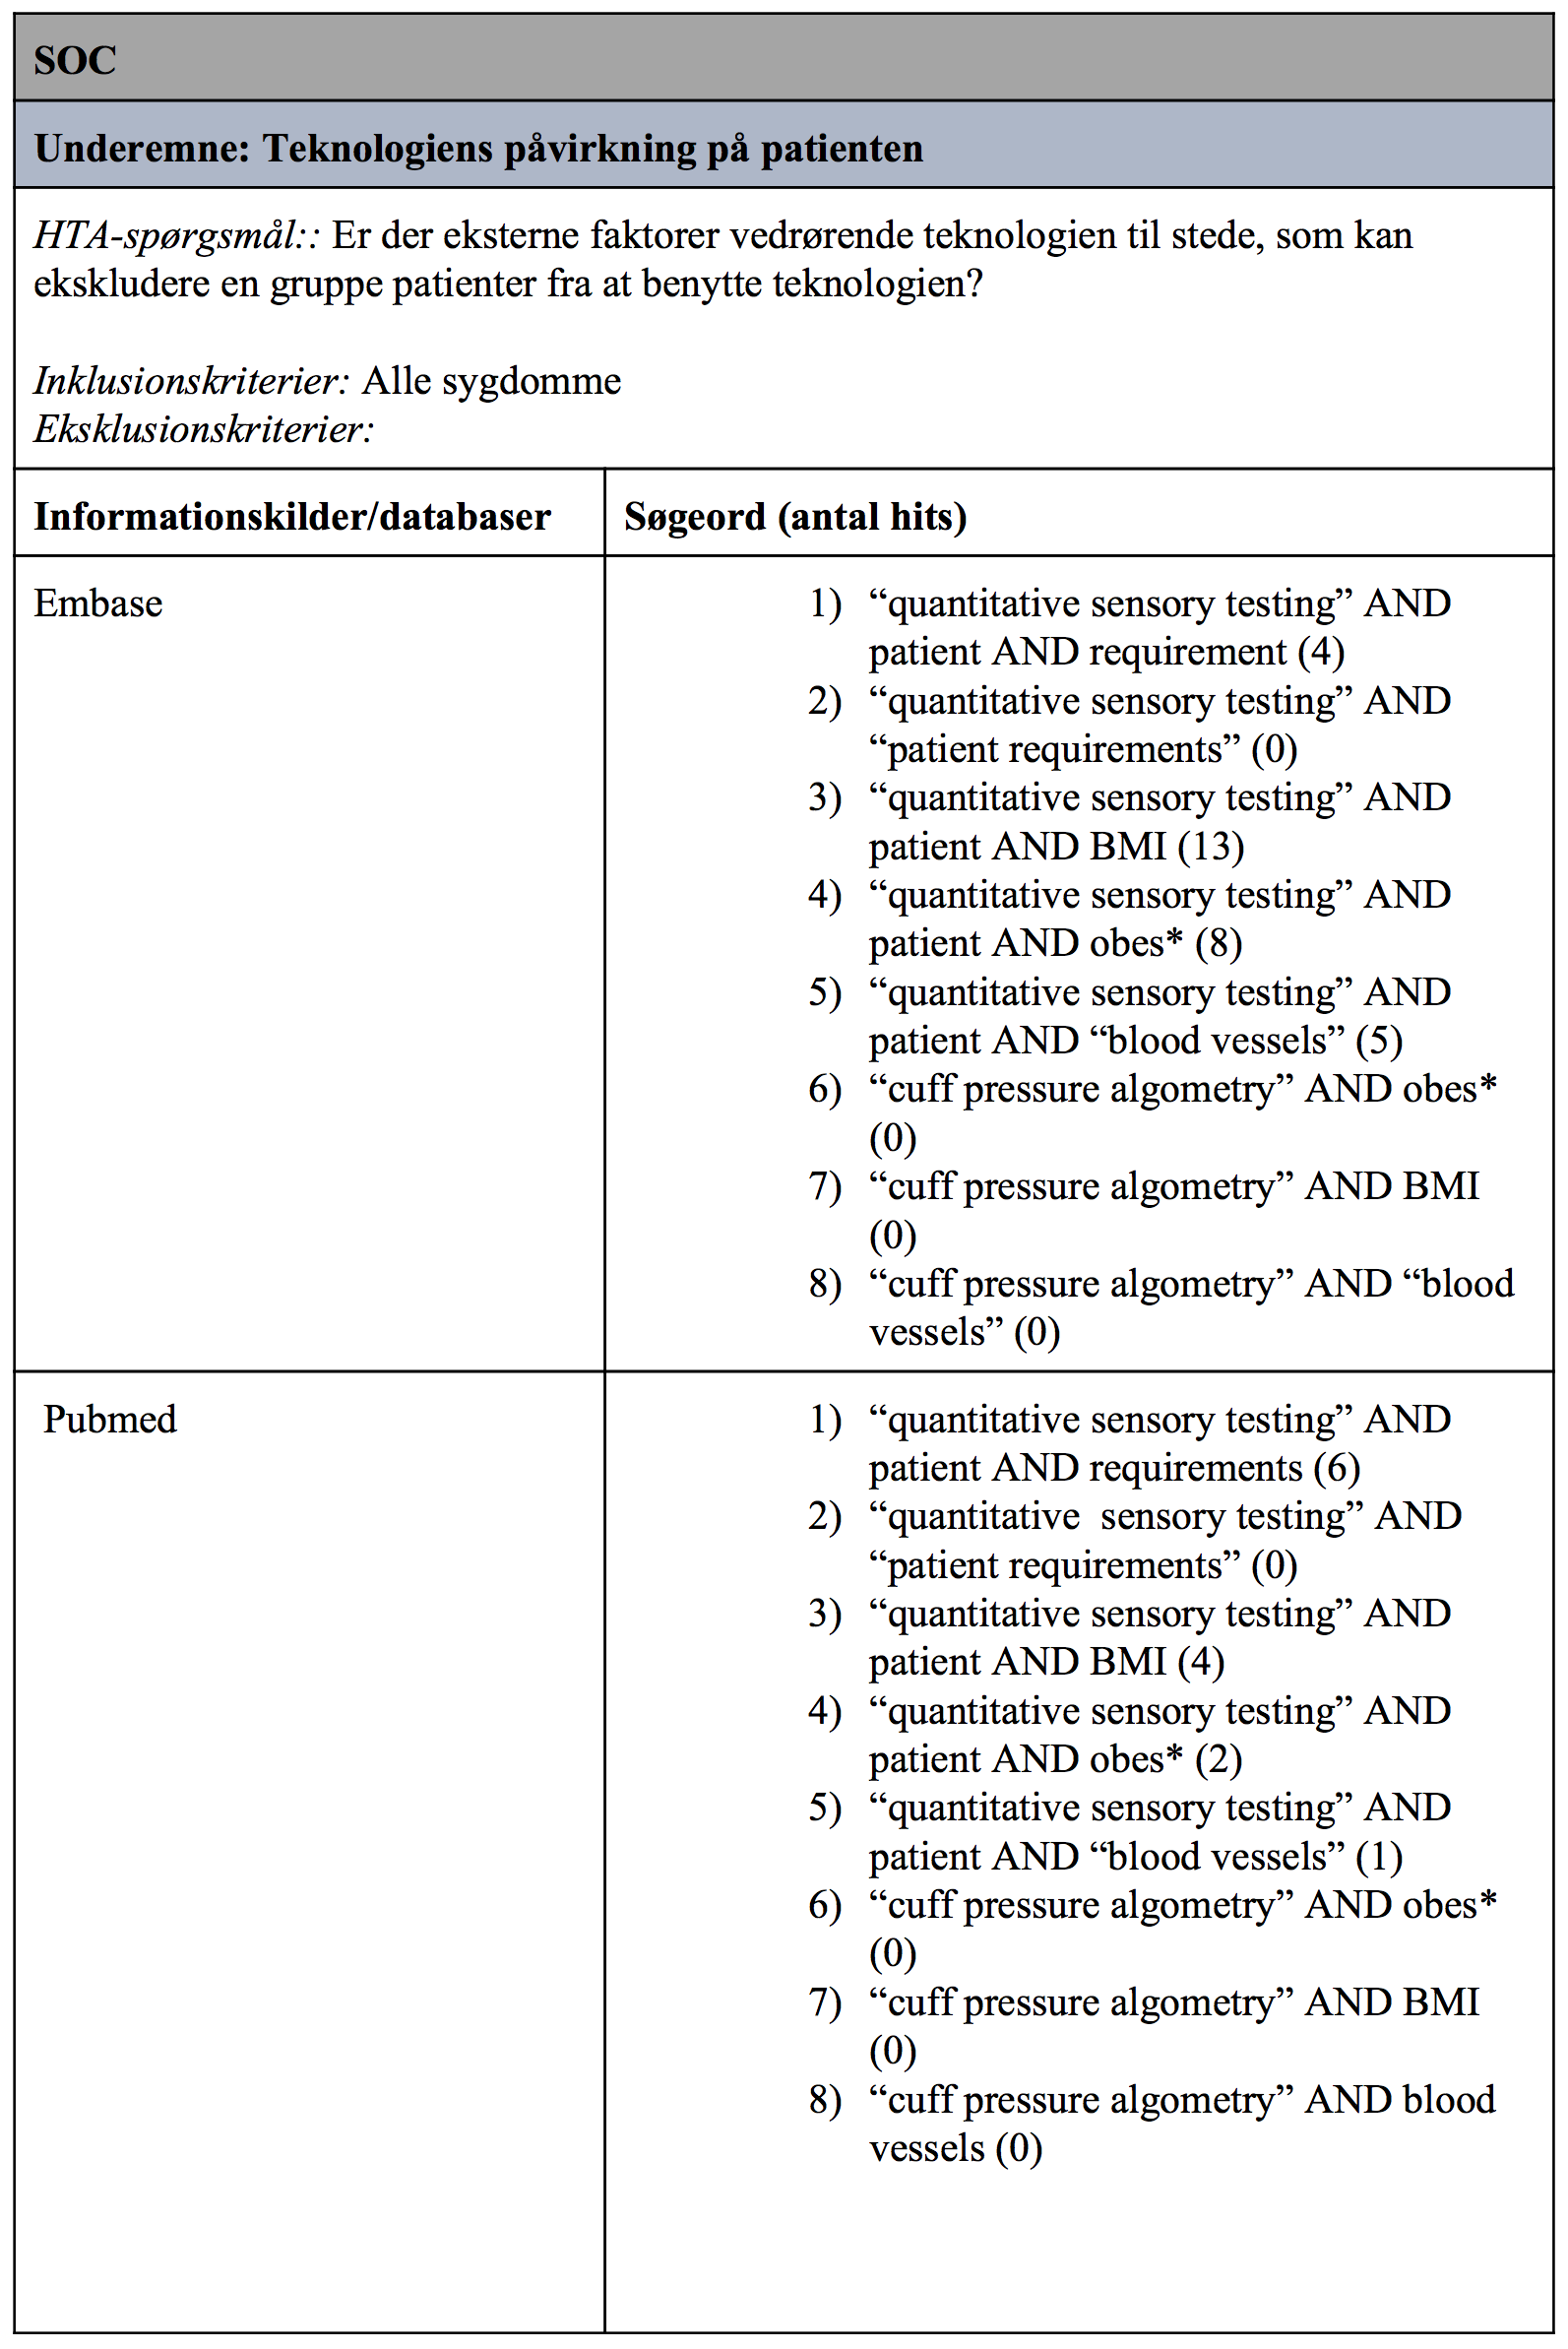
\includegraphics[width=0.8\textwidth]{rapportAfsnit/qBilag/sogninger/SOC1}

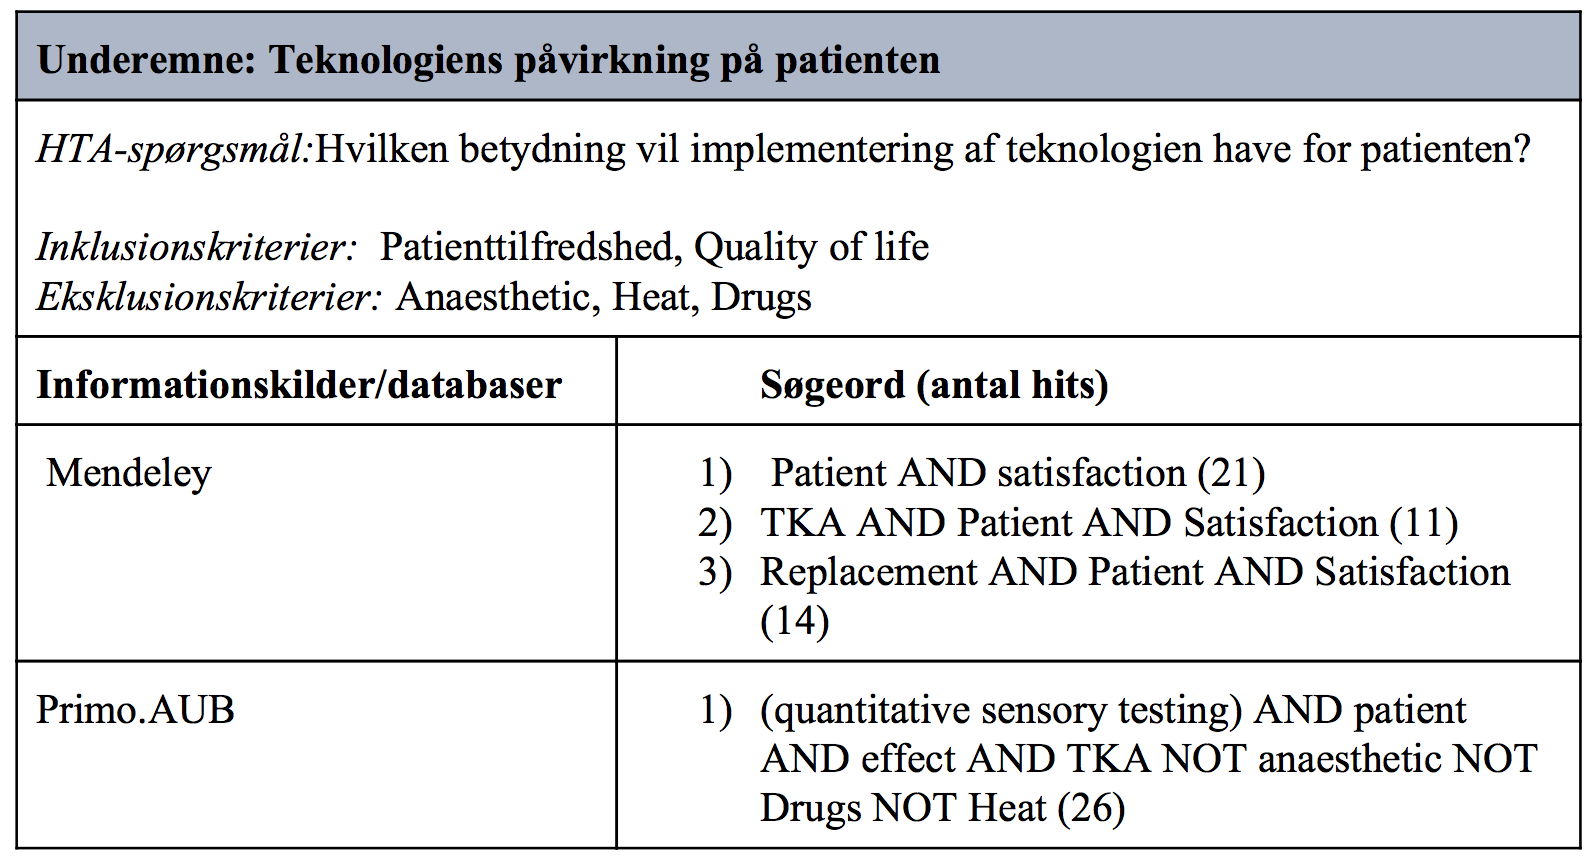
\includegraphics[width=0.8\textwidth]{rapportAfsnit/qBilag/sogninger/SOC2}

\section{ETH}\label{ETH_sog}
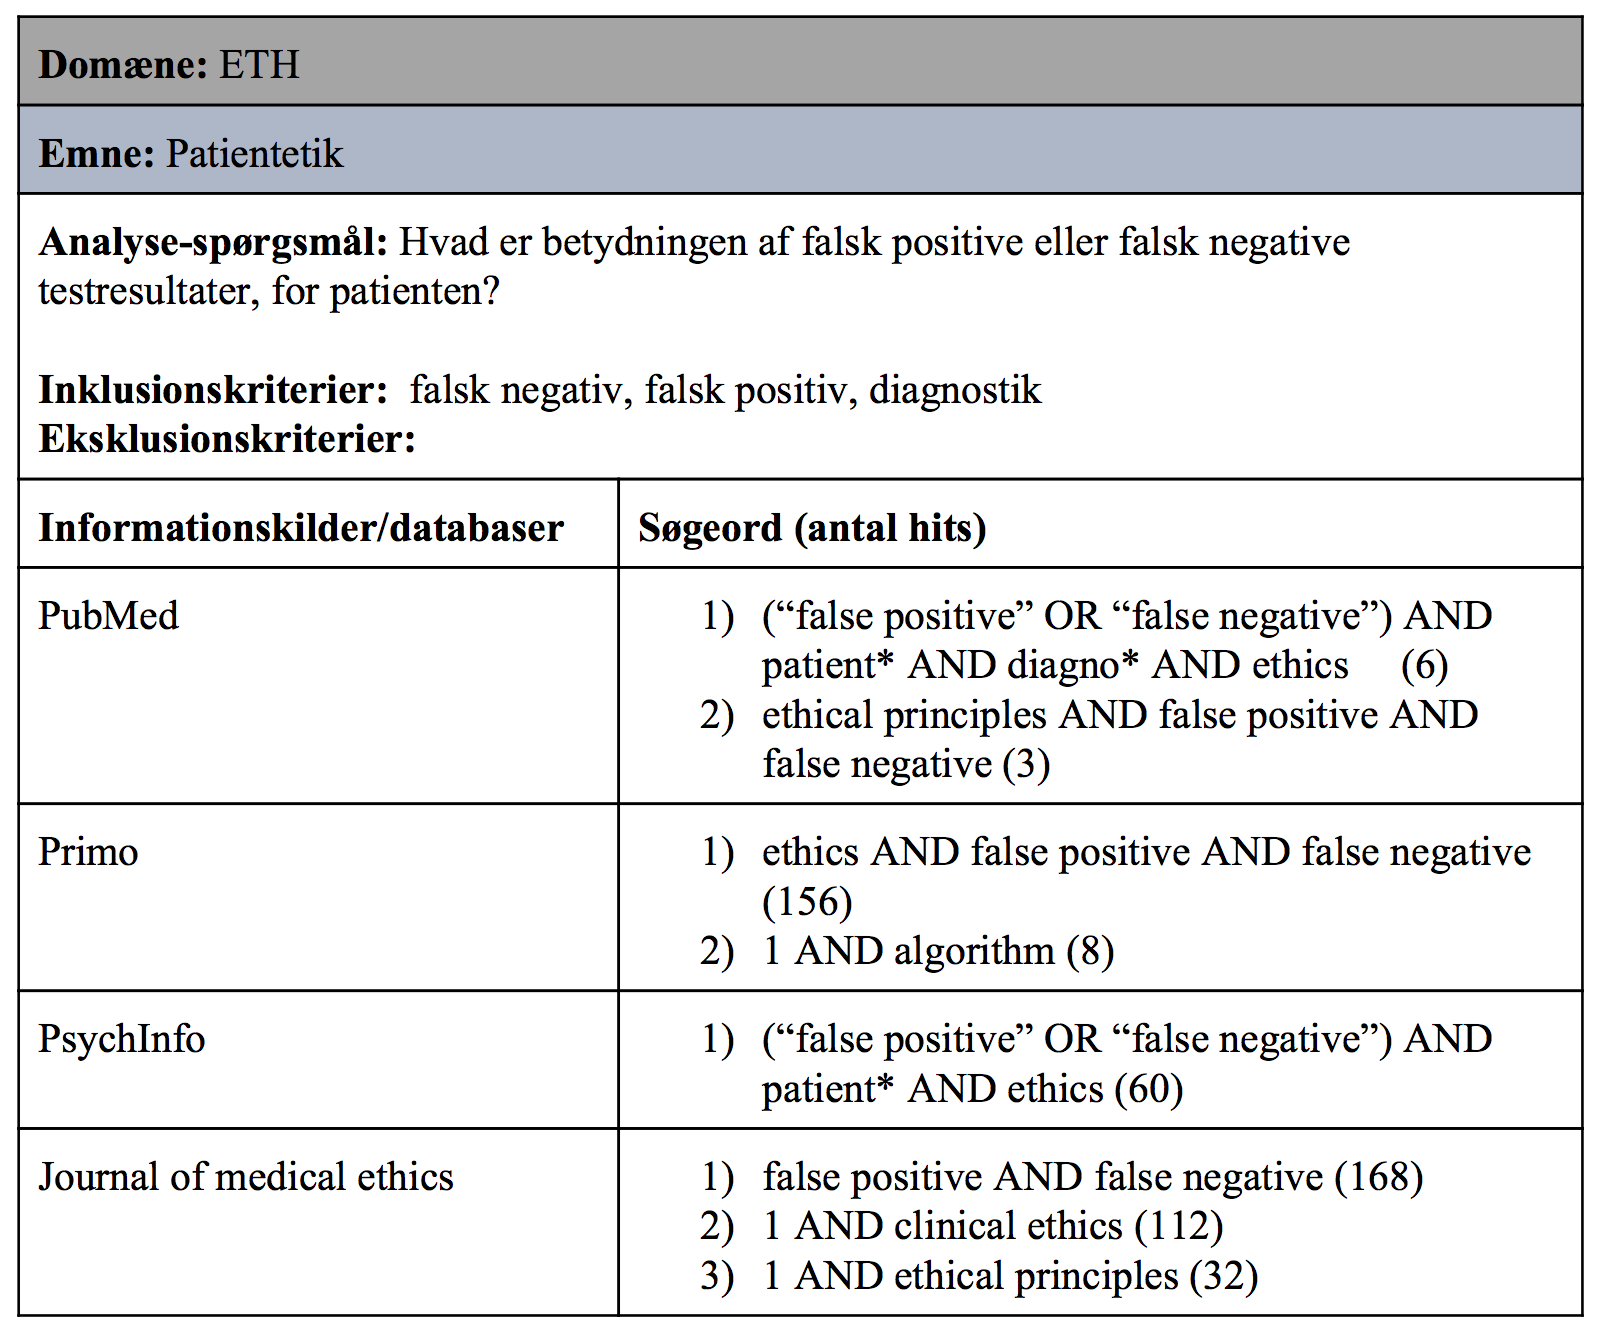
\includegraphics[width=0.8\textwidth]{rapportAfsnit/qBilag/sogninger/ETH1}

\section{ECO}\label{ECO_sog}
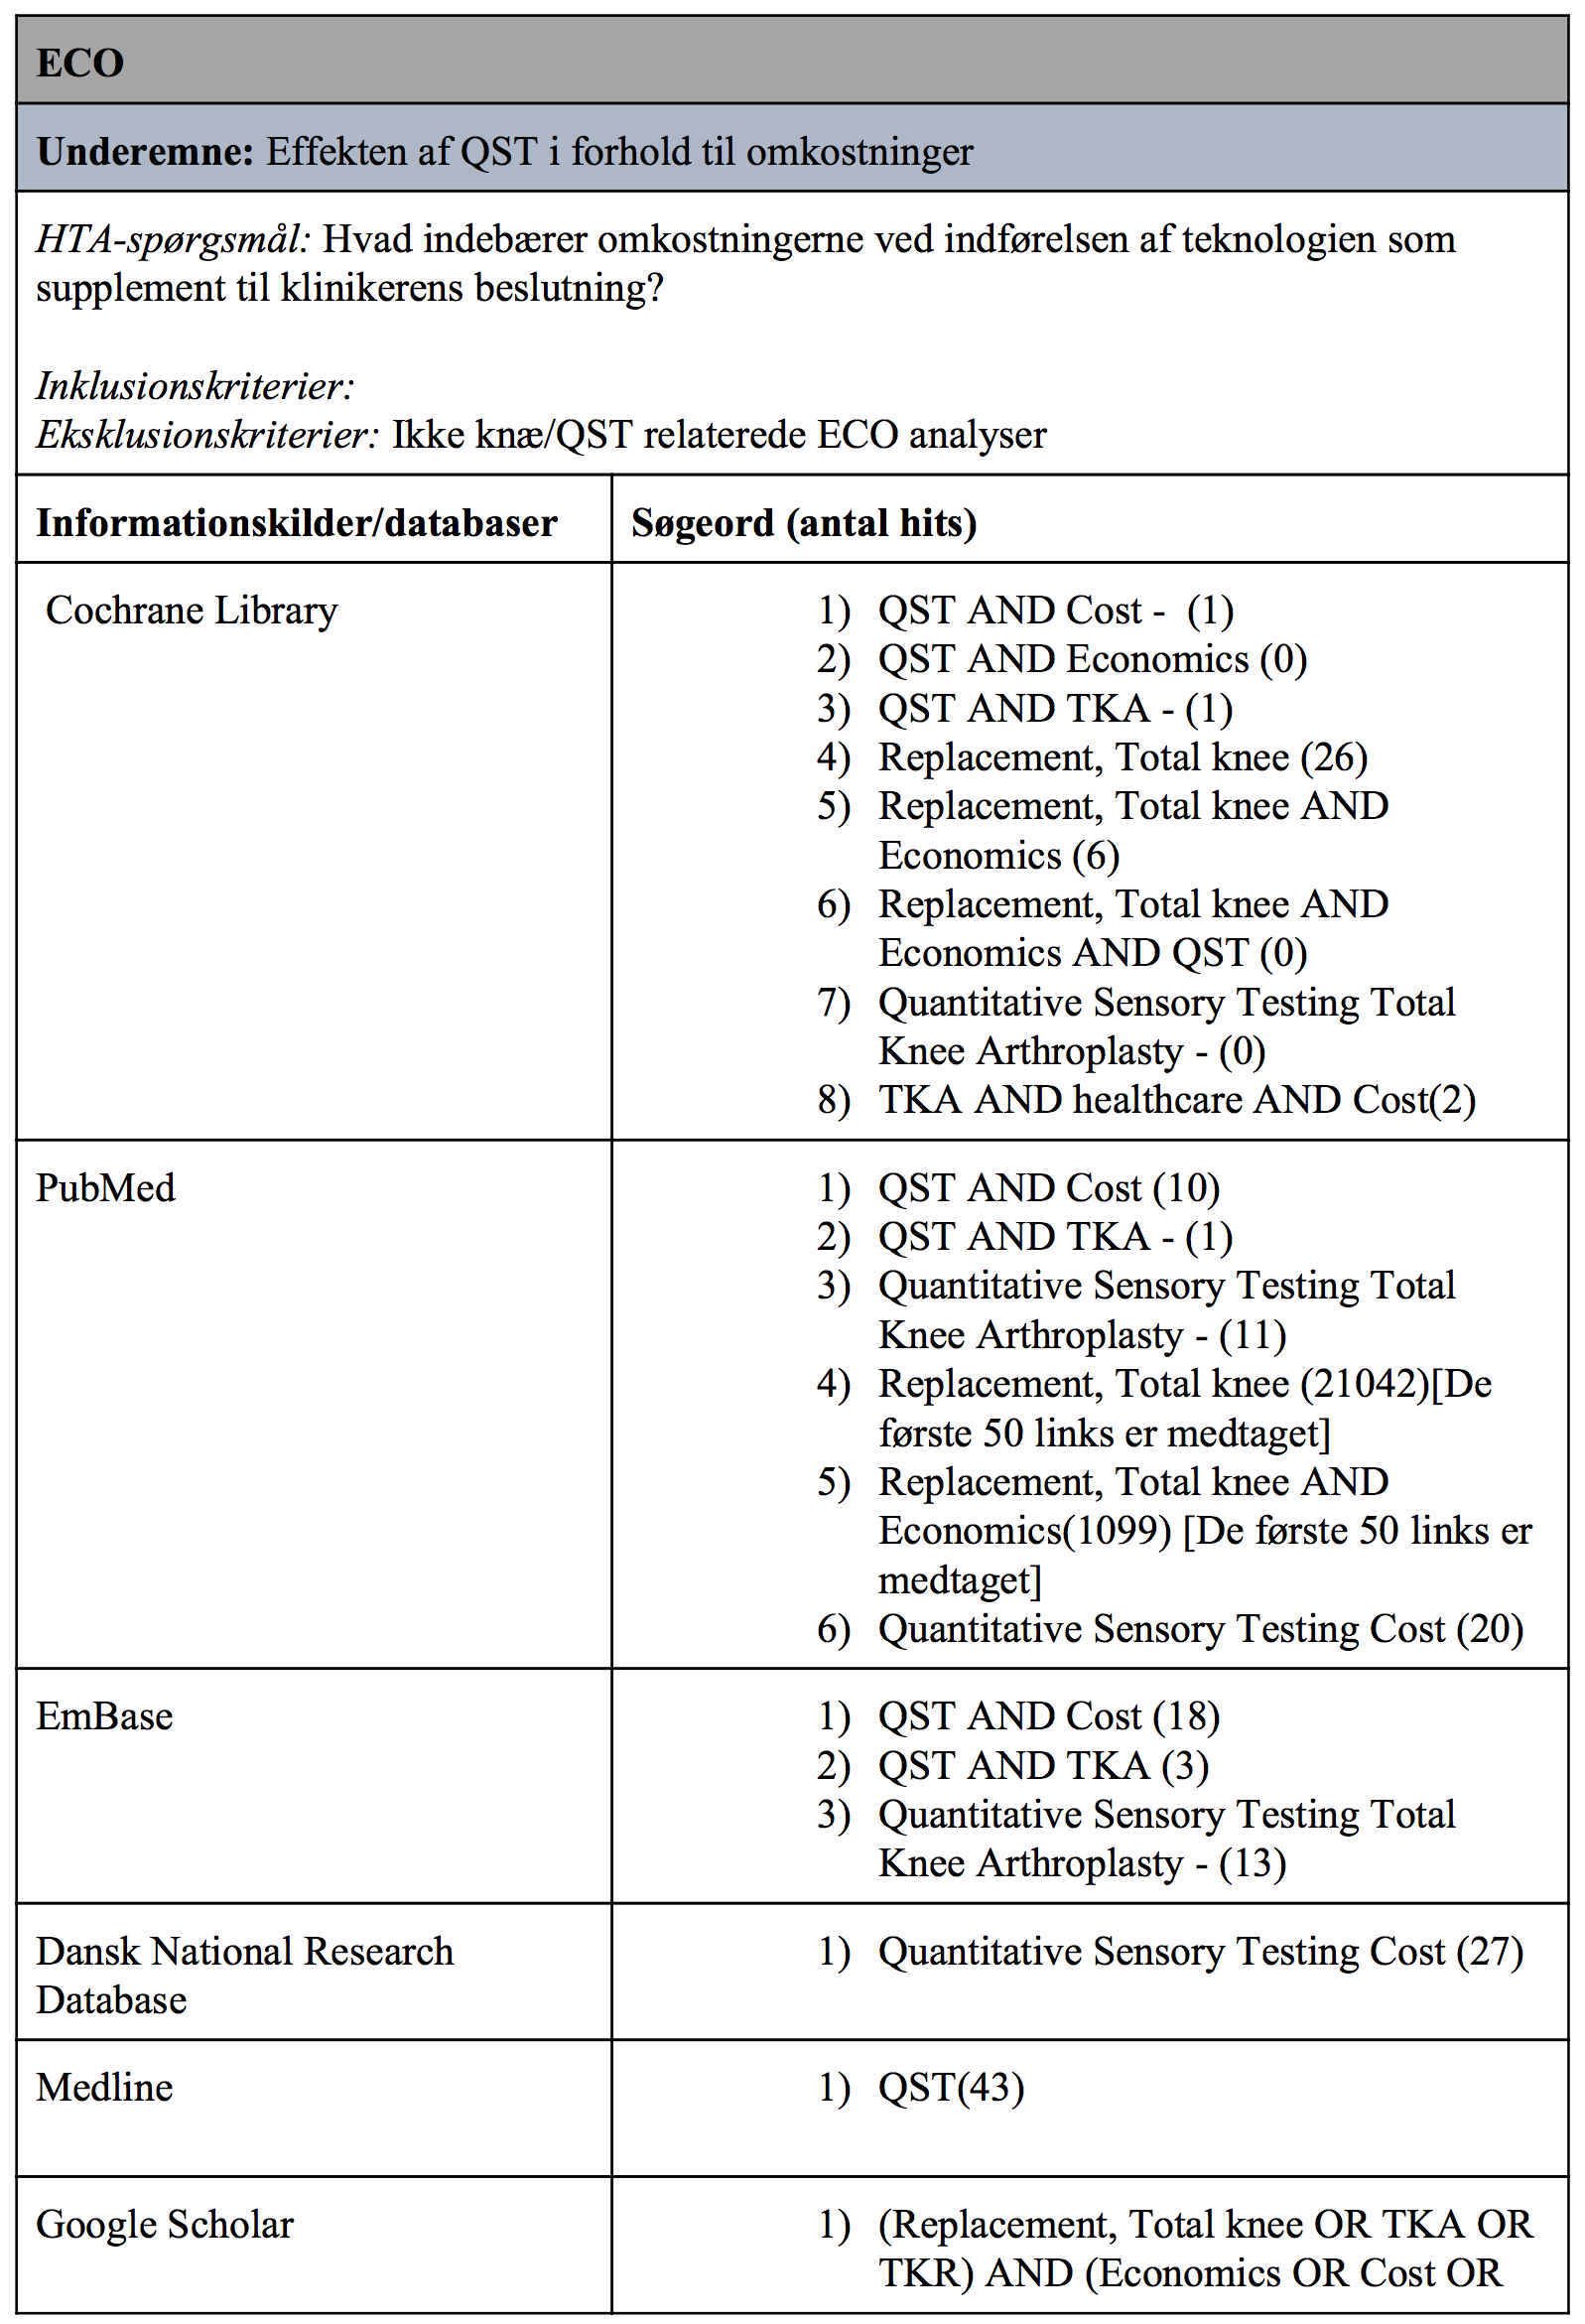
\includegraphics[width=0.8\textwidth]{rapportAfsnit/qBilag/sogninger/ECO1}

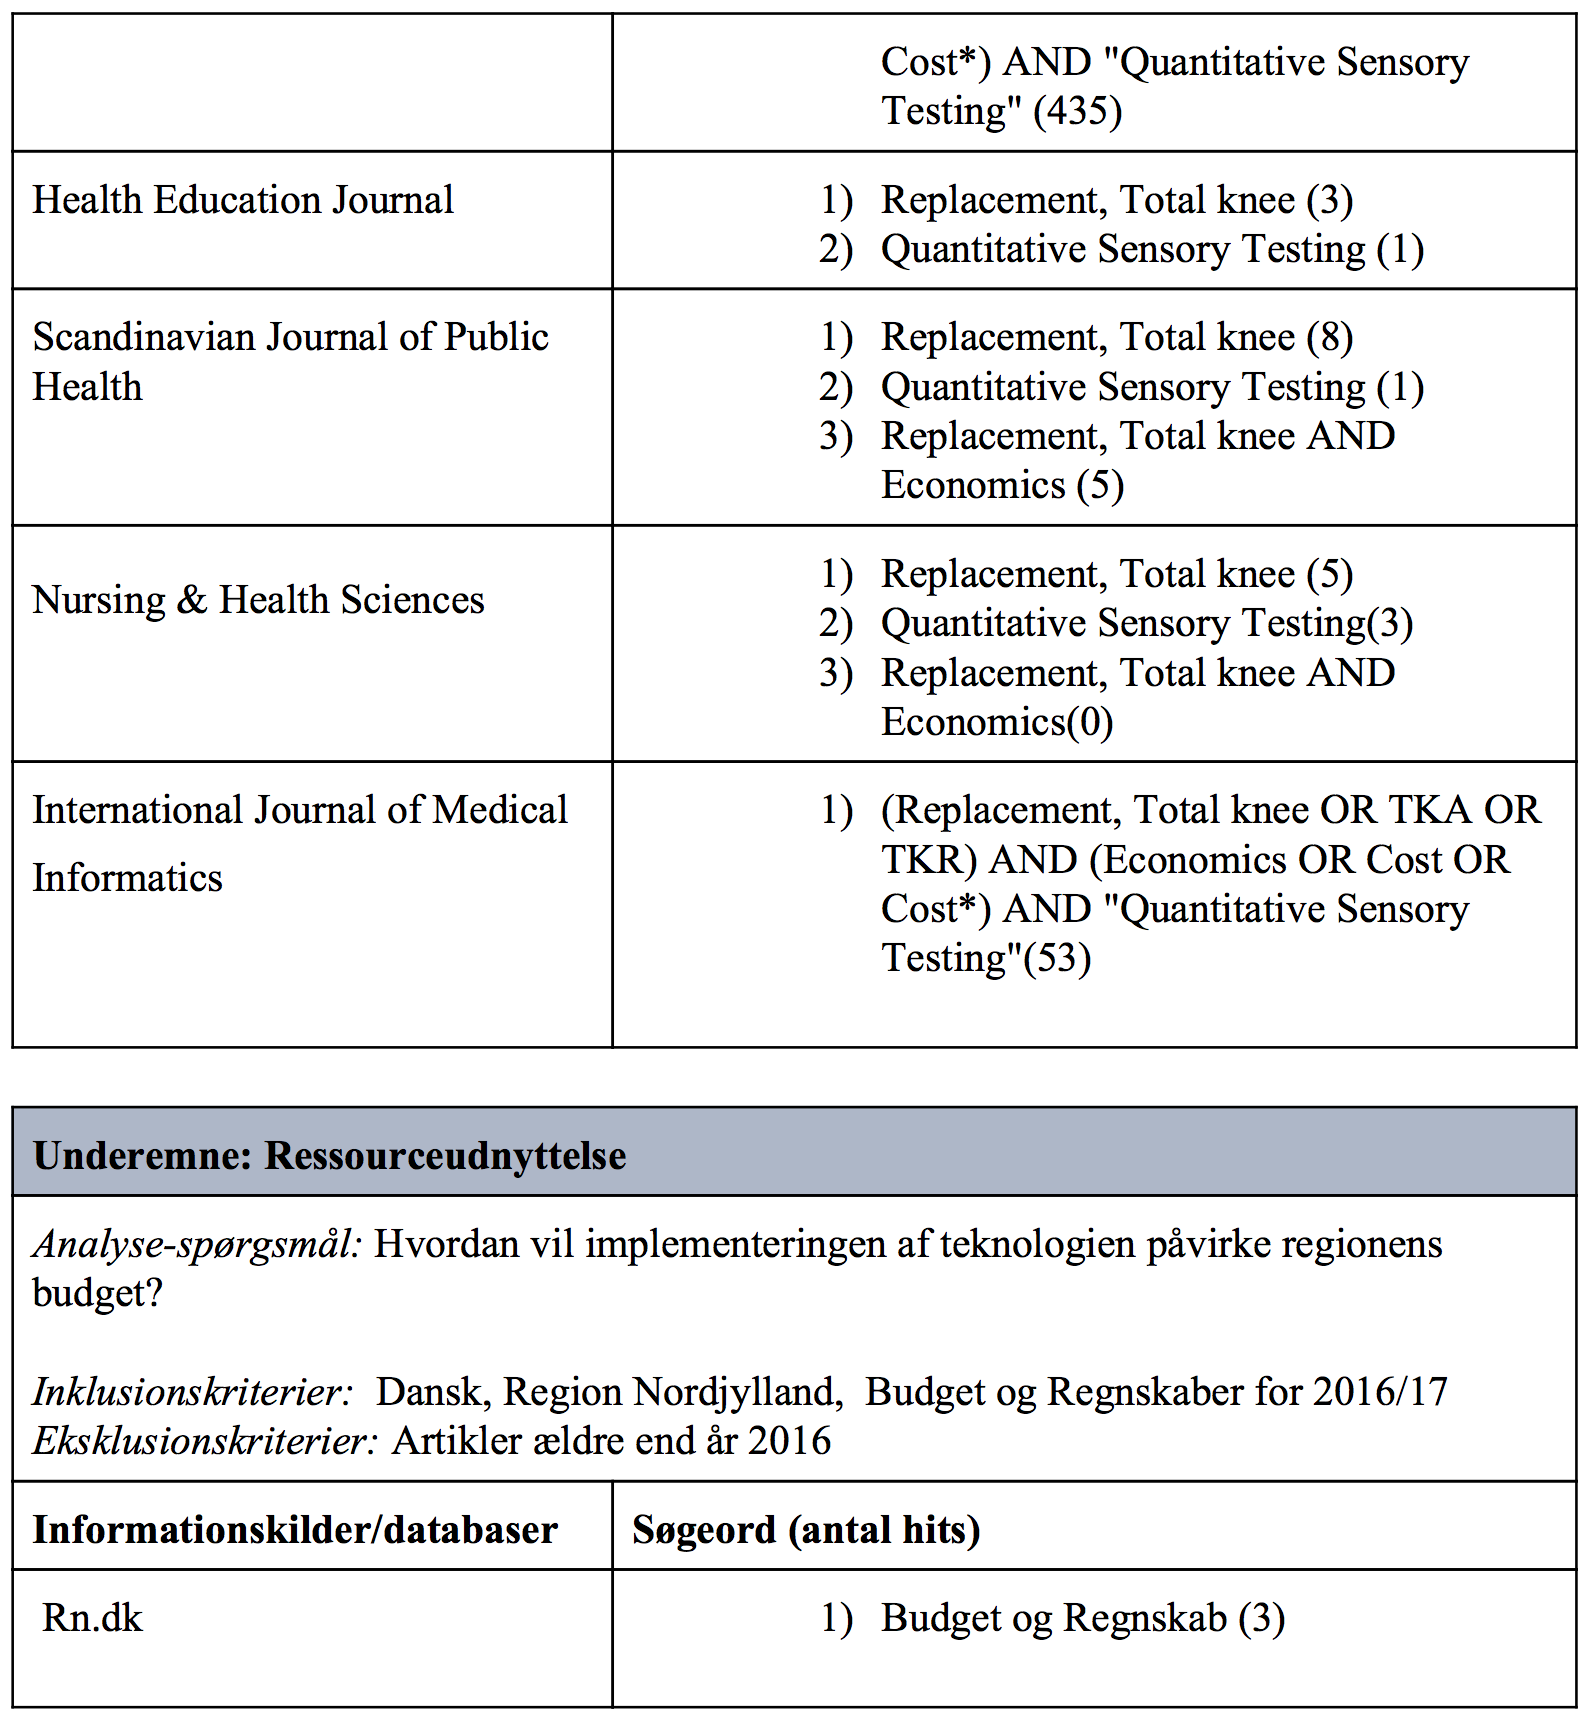
\includegraphics[width=0.8\textwidth]{rapportAfsnit/qBilag/sogninger/ECO2}







%\begin{table}[H]
%\centering
%\caption{My caption}
%\label{my-label}
%\begin{tabular}{|ll|}
%\hline
%\rowcolor[HTML]{656565} 
%{\color[HTML]{000000} \textbf{Problemanalyse}}                                     & {\color[HTML]{656565} }                              \\ \hline
%\textit{Fokuseret sprøgsmål:}                                                      &                                                      \\
%                                                                                   &                                                      \\
%\textit{Inklusion- og ekslusionskriterier:}                                        &                                                      \\
%\textit{Inklusion:}                                                                &                                                      \\
%\textit{Eksklusion:}                                                               &                                                      \\ \hline
%\rowcolor[HTML]{C0C0C0} 
%{\color[HTML]{000000} \textbf{Underemne: Indledning og initierende problem}}       & {\color[HTML]{C0C0C0} }                              \\ \hline
%\textit{Fokuseret spørgsmål:}                                                      &                                                      \\
%                                                                                   &                                                      \\
%\textit{Inklusionskriterier:}                                                      &                                                      \\
%\textit{Eksklusionskriterier:}                                                     &                                                      \\ \hline
%\multicolumn{1}{|l|}{{\color[HTML]{000000} \textbf{Informationskilder/databaser}}} & {\color[HTML]{000000} \textbf{Søgeord (antal hits)}} \\ \hline
%\multicolumn{1}{|l|}{}                                                             &                                                      \\ \hline
%\rowcolor[HTML]{C0C0C0} 
%{\color[HTML]{000000} \textbf{Underemne: Indledning og initierende problem}}       & {\color[HTML]{000000} }                              \\ \hline
%\textit{Fokuseret spørgsmål:}                                                      &                                                      \\
%                                                                                   &                                                      \\
%\textit{Inklusionskriterier:}                                                      &                                                      \\
%\textit{Eksklusionskriterier:}                                                     &                                                      \\ \hline
%\end{tabular}
%\end{table}